Estos son los resultados de estos experimentos en cuestión\\ 

Empezaremos mostrando los resultados de los algoritmos de ordenamiento de arreglos (Sort, MergeSort y QuickSort) 

\begin{figure}[H]
    \centering
    \begin{minipage}[t]{0.5\textwidth}
        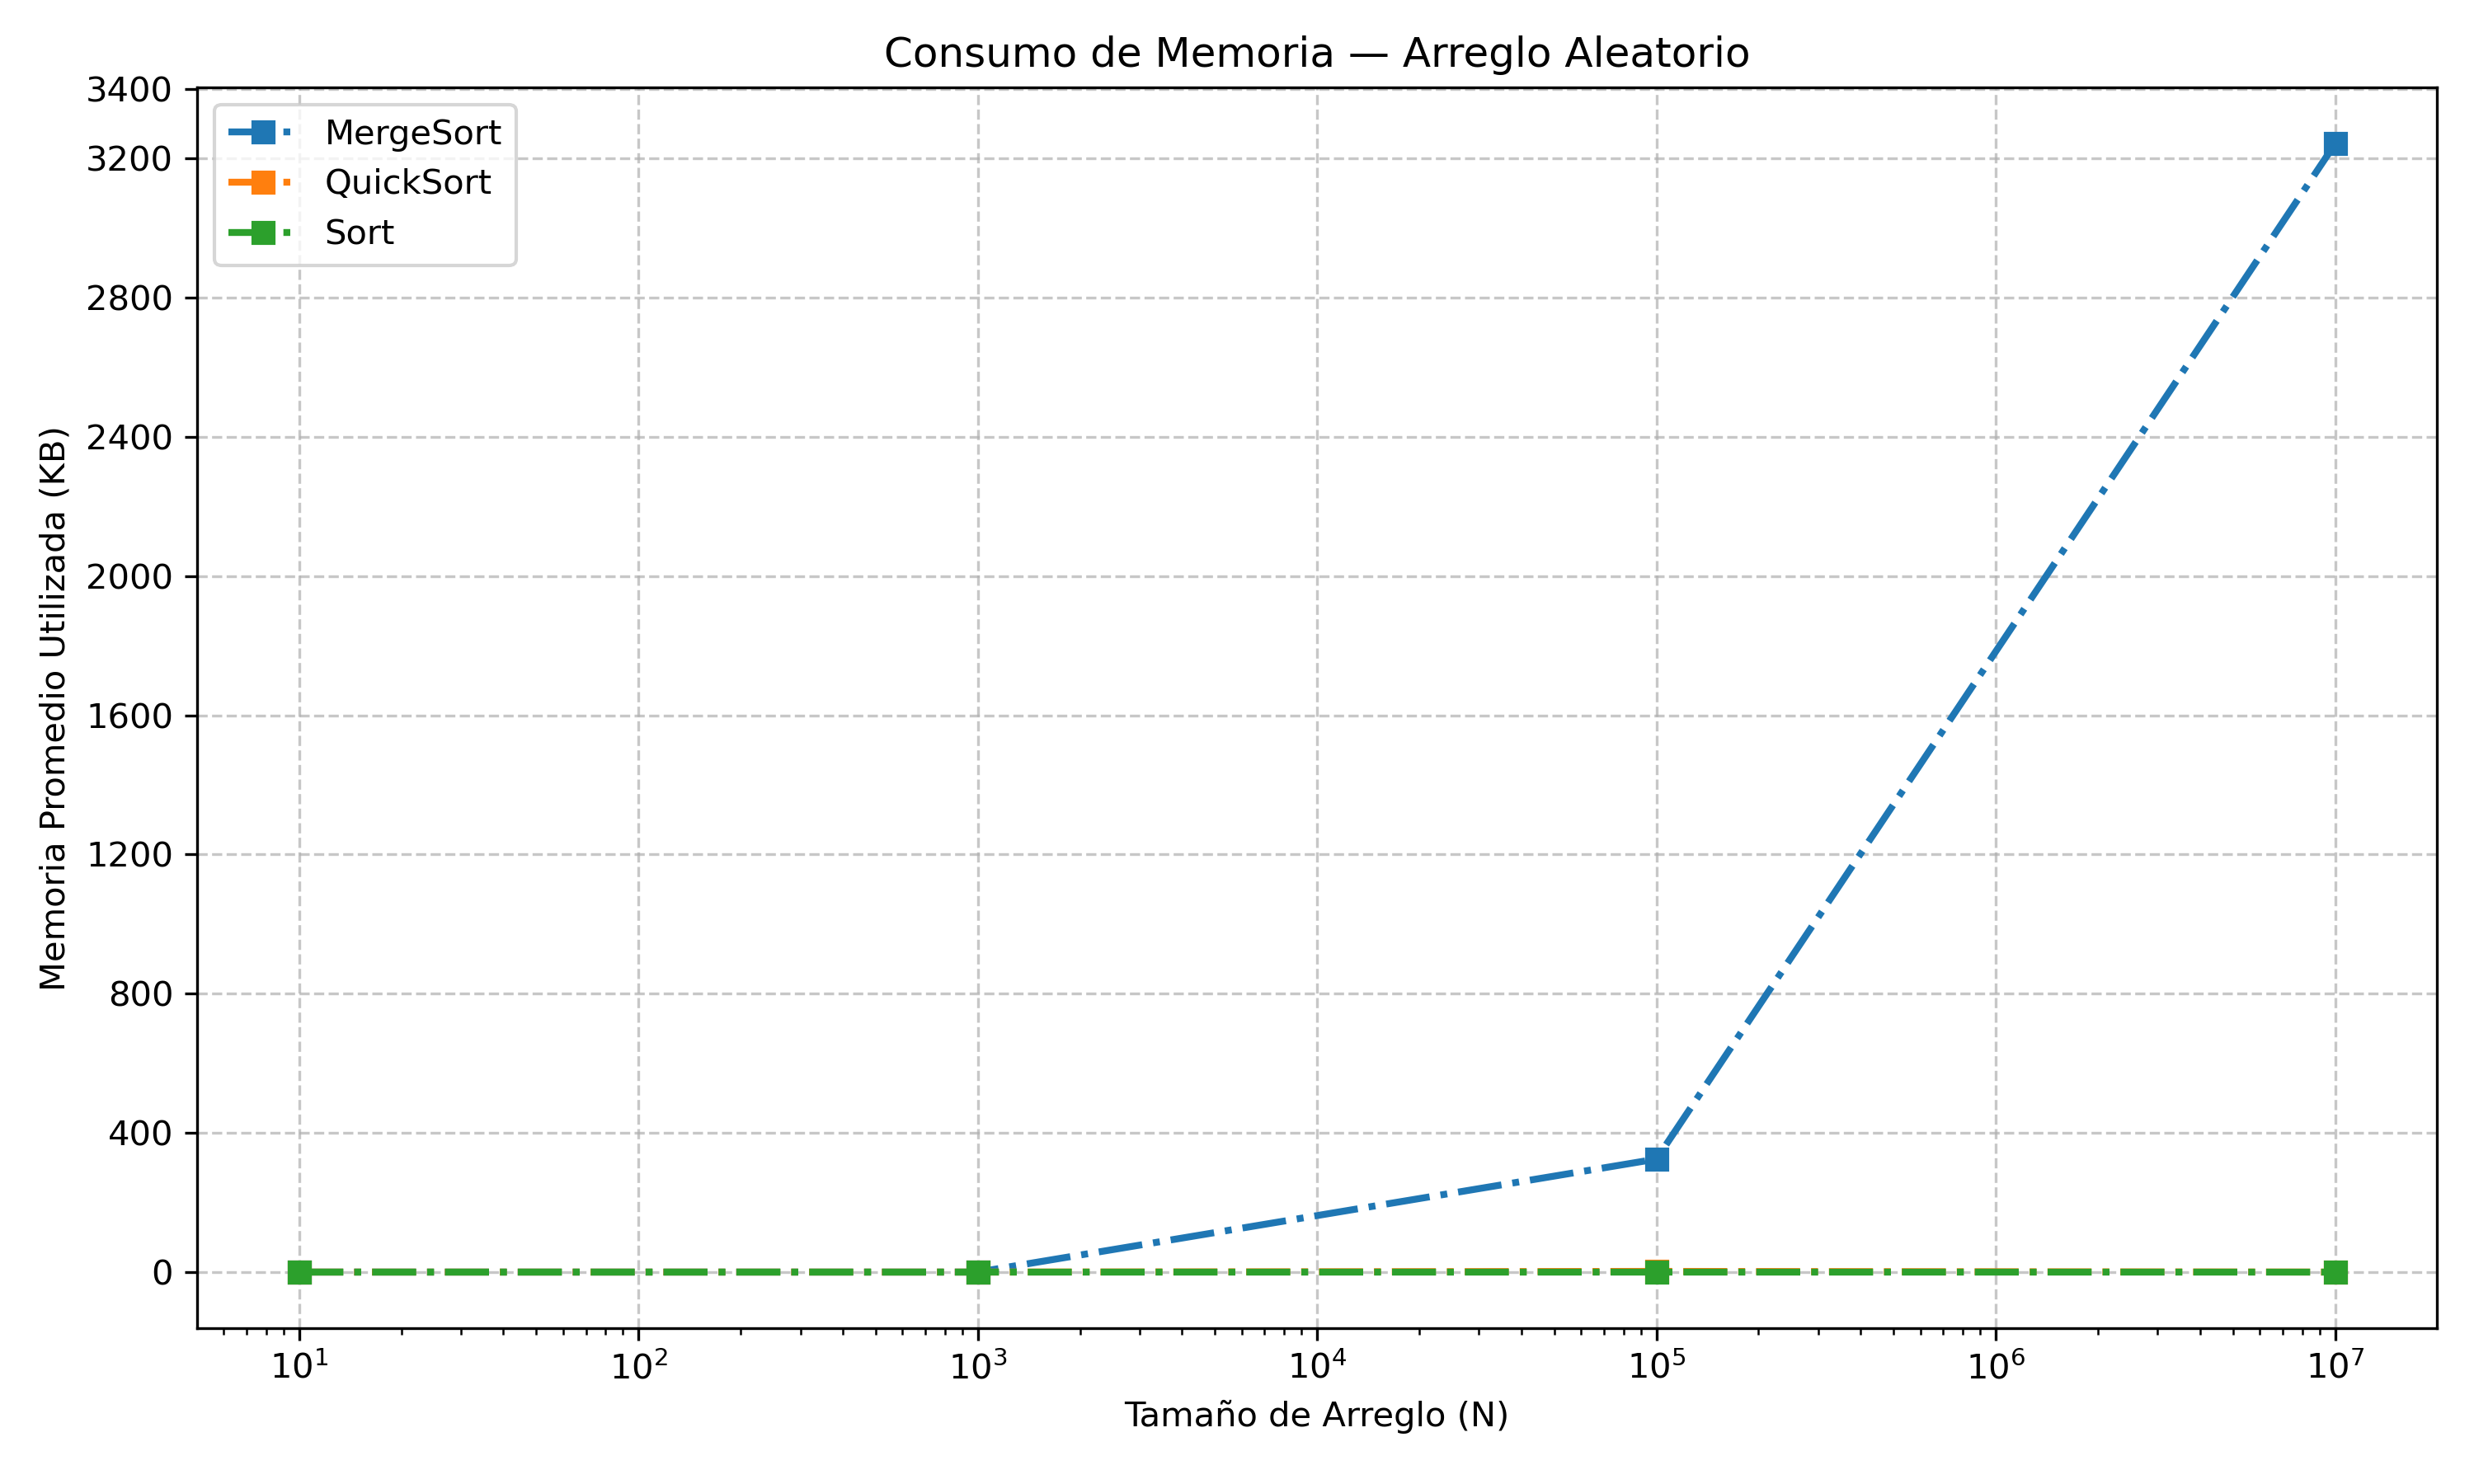
\includegraphics[width=\textwidth]{../code/sorting/data/plots/memoria_aleatorio.png}
    \end{minipage}%
    \begin{minipage}[t]{0.5\textwidth}
        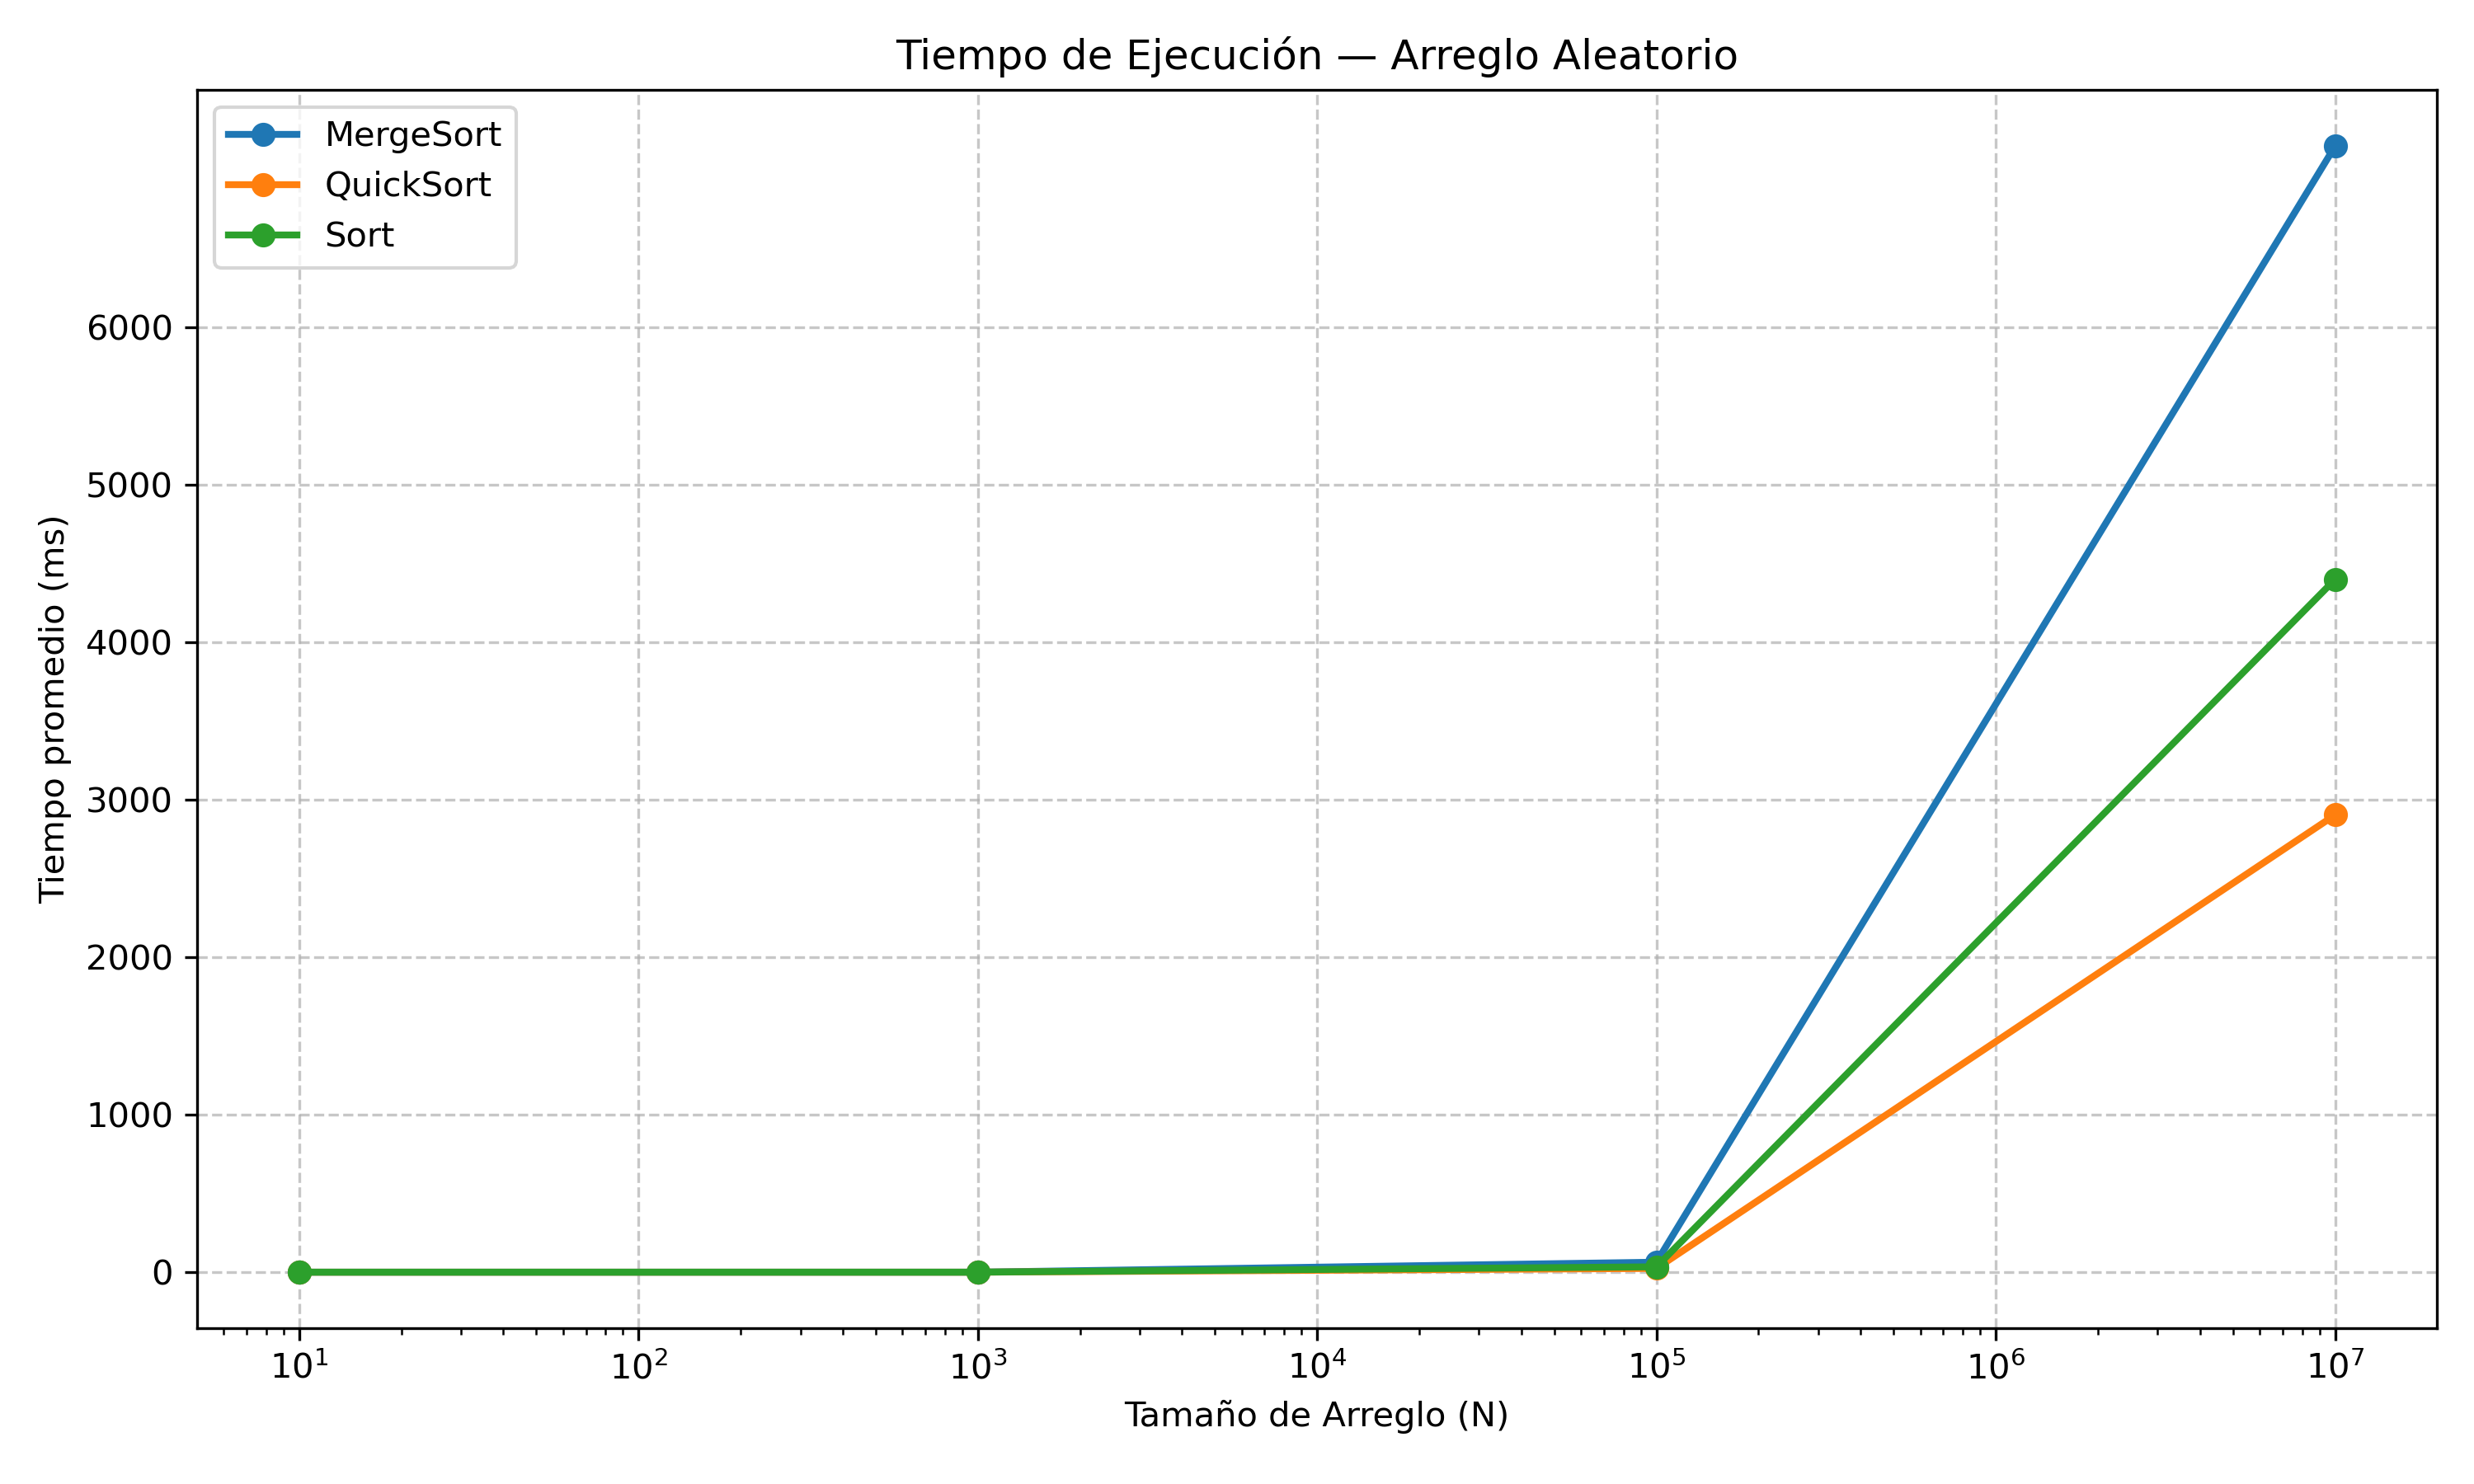
\includegraphics[width=\textwidth]{../code/sorting/data/plots/tiempo_aleatorio.png}
    \end{minipage}%
    \caption{Comparación del tiempo de ejecución y consumo de memoria de arreglos aleatorios por cada algoritmo}
    \label{fig:grafico_aleatorio}
\end{figure}

En Mergesort observamos que posee el mayor consumo de memoria debido principalmente al enfoque de "dividir y conquistar", al usar arreglos auxiliares durante las comparaciones, junto con el enfoque recursivo da como resultado un consumo de memoria mayor al resto de algoritmos. 

Quicksort y sort presentan consumos de memoria mucho más bajos, incluso en los arreglos más grandes debido a que poseen un enfoque totalmente distinto que no depende del uso de arreglos auxiliares como mergesort, ahorrando mucho en este aspecto. 

En cuanto a tiempos, todos los algoritmos resultaron ser rápidos en arreglos de hasta 100000, pero cuando llegamos al tamaño máximo en el dataset estos escalan notoriamente, siendo mergesort el más tardío de los 3 en promedio de todos los casos, y con una diferencia notoria. 

\begin{figure}[H]
    \centering
    \begin{minipage}[t]{0.5\textwidth}
        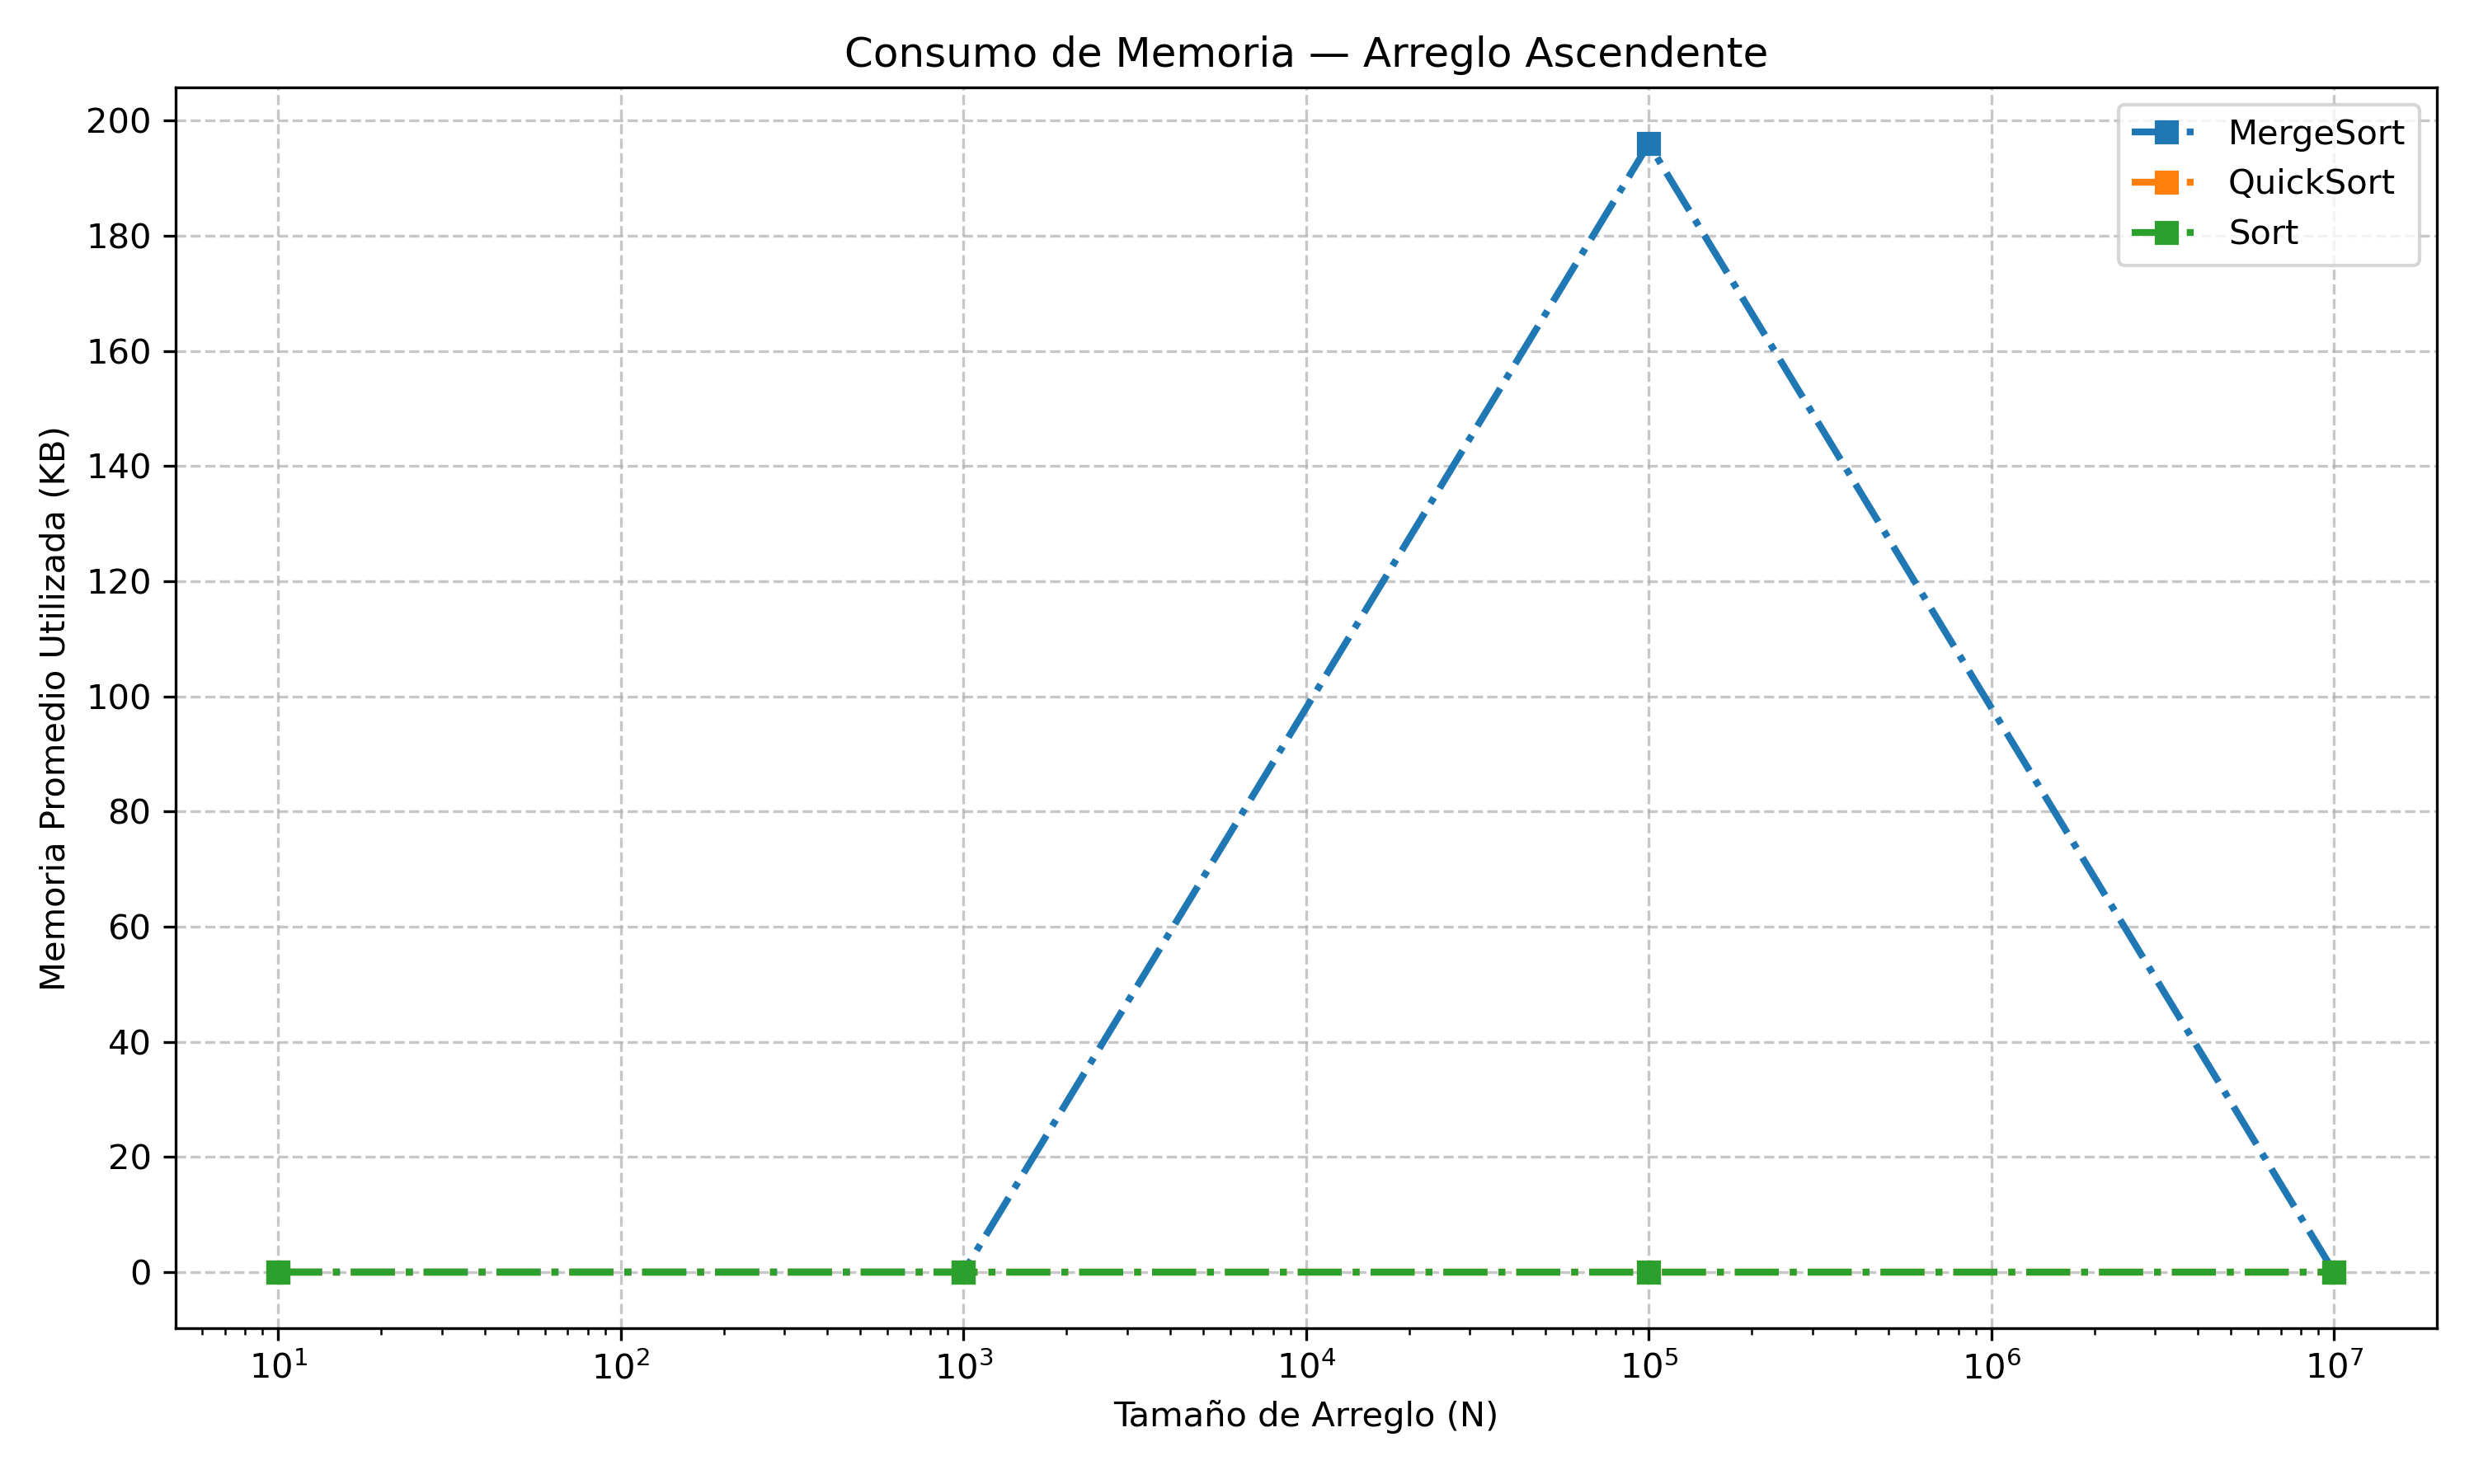
\includegraphics[width=\textwidth]{../code/sorting/data/plots/memoria_ascendente.png}
    \end{minipage}%
    \begin{minipage}[t]{0.5\textwidth}
        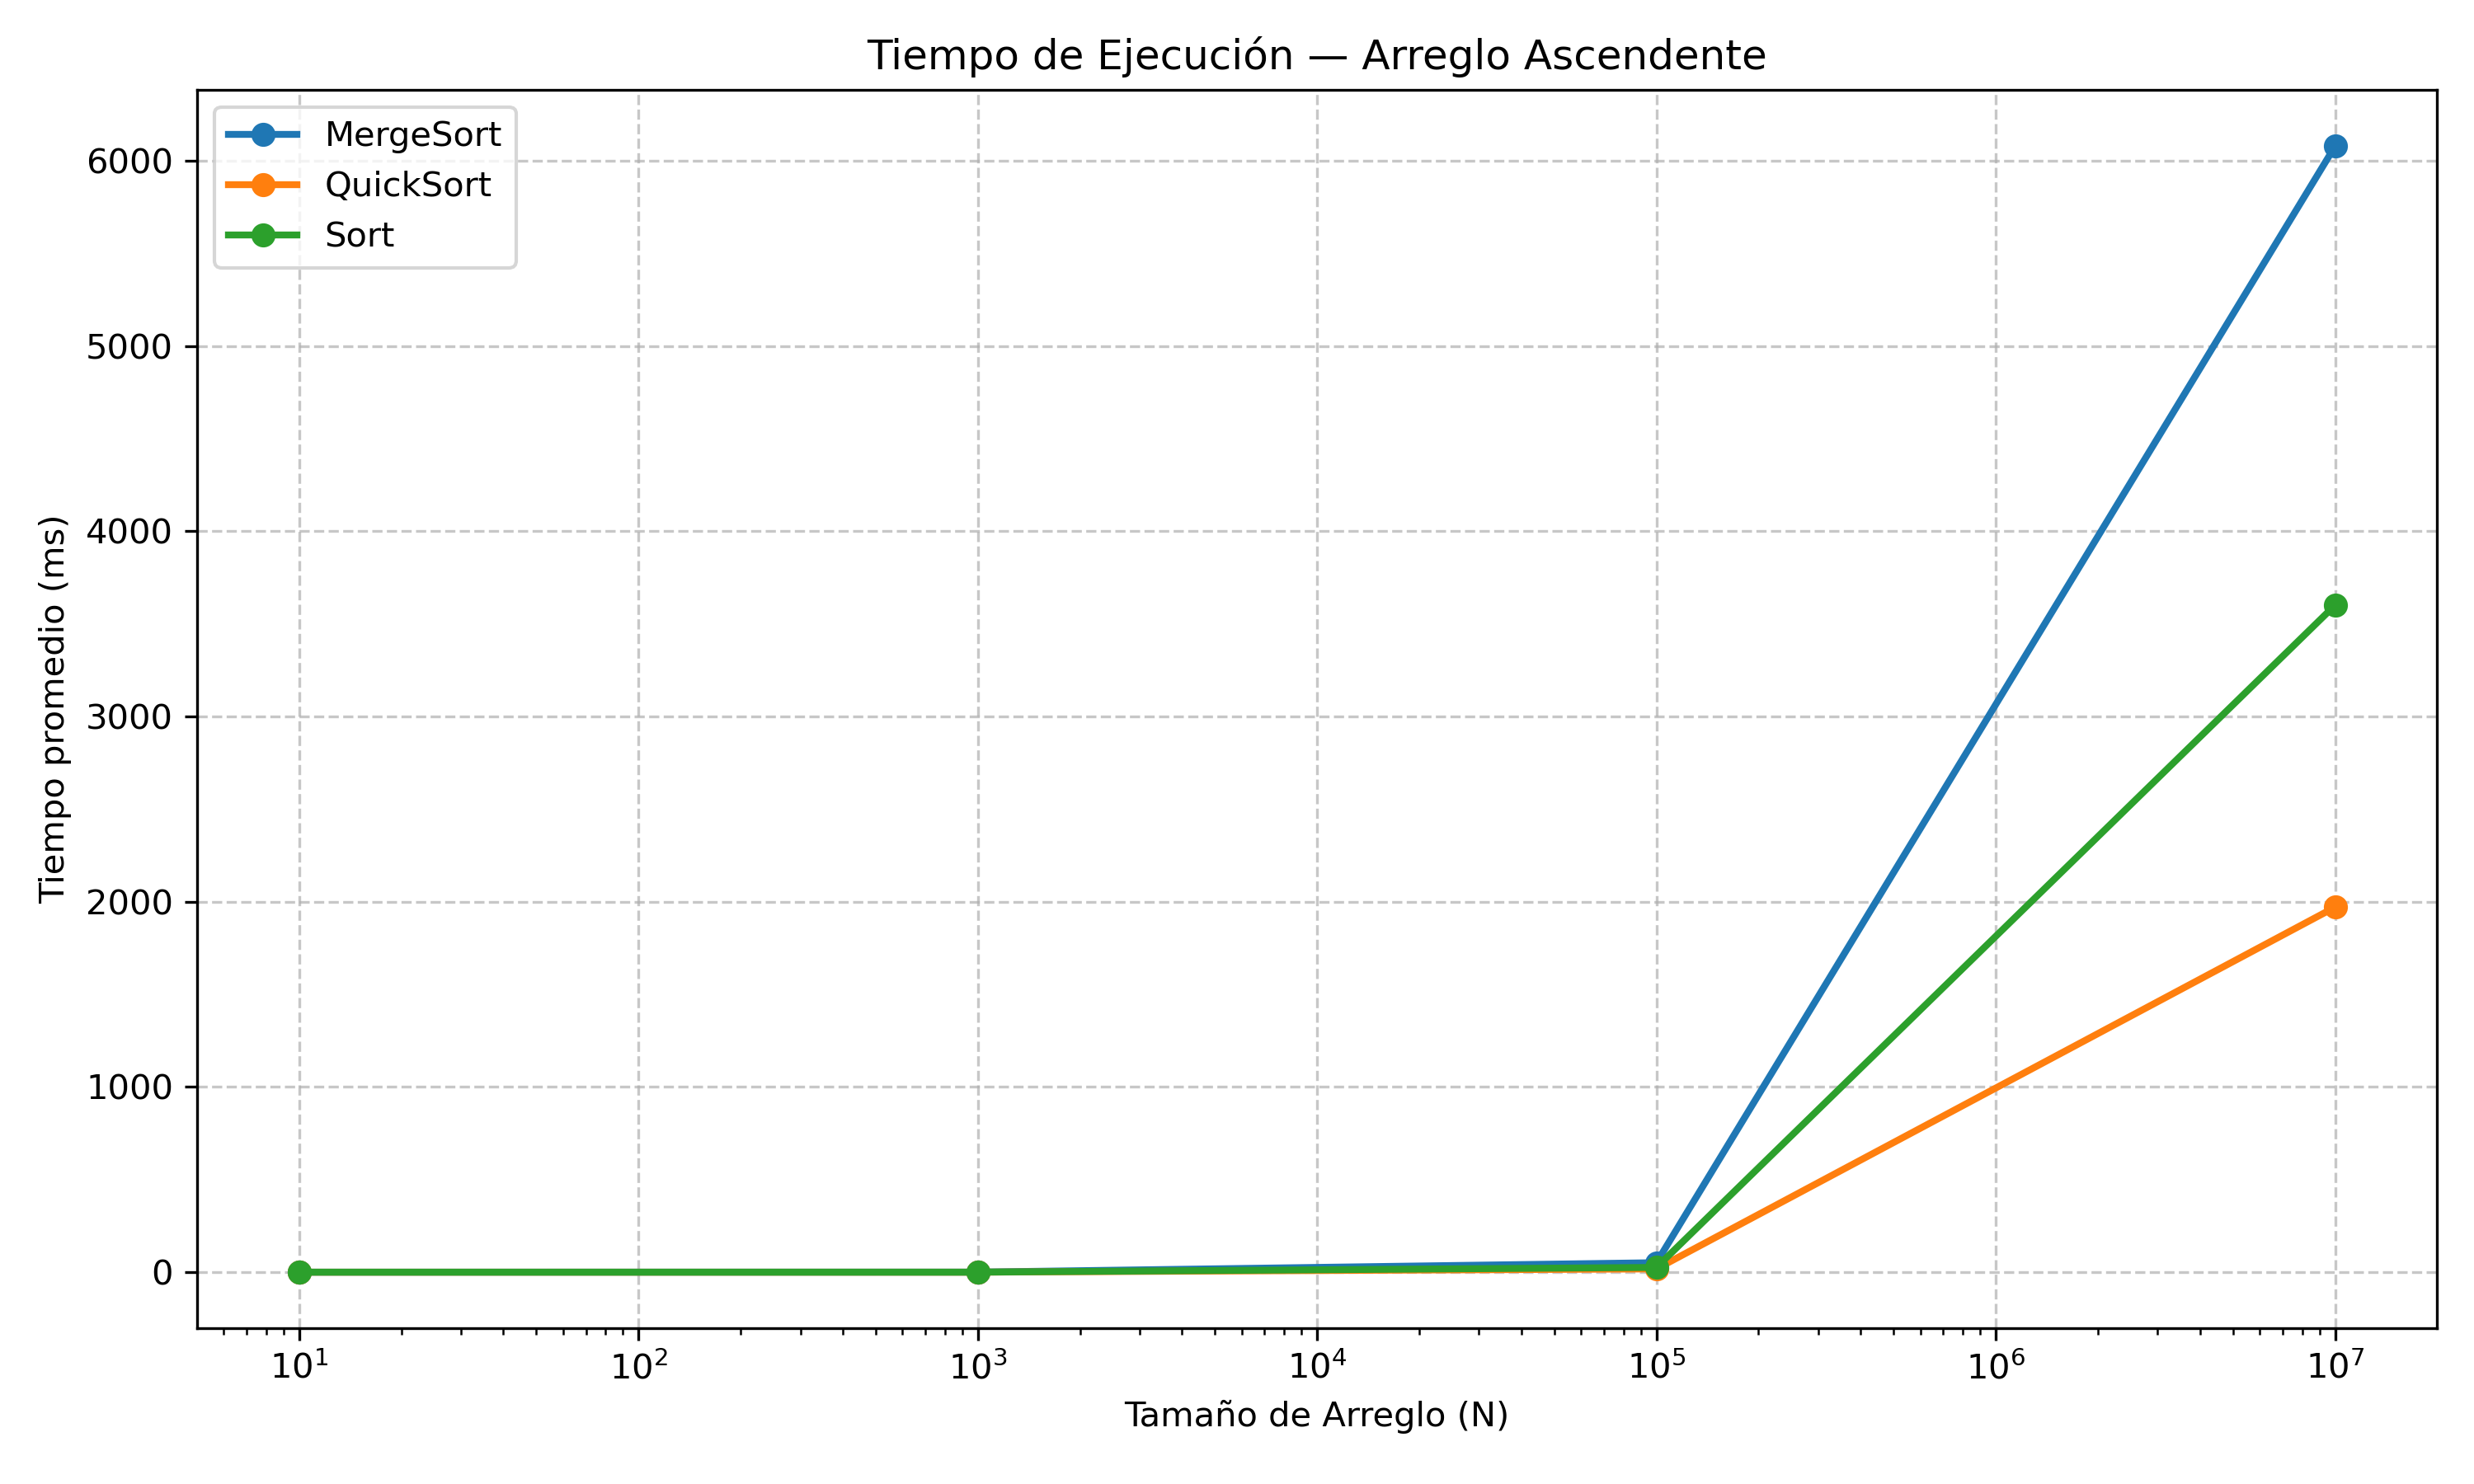
\includegraphics[width=\textwidth]{../code/sorting/data/plots/tiempo_ascendente.png}
    \end{minipage}%
    \caption{Comparación del tiempo de ejecución y consumo de memoria de arreglos ascendentes por cada algoritmo}
    \label{fig:grafico_ascendente}
\end{figure}

En lo que respecta al consumo de memoria observamos que en Mergesort ocurre algo muy extraño, y es que presenta su mayor consumo de memoria en los arreglos de tamaño 100000 en vez de los de 10 millones, se ha probado con otras formas de medición de memoria y todos arrojan el mismo resultado. Lo más probable es que esto se deba en parte al funcionamiento de la gestión de memoria del SO. 

En el caso de los otros algoritmos, estos mantienen un consumo bajo de memoria dado el enfoque de estos, por lo que se esperaba que MergeSort fuera el que destacara en este aspecto. 

En cuanto al tiempo de ejecución, el escenario es muy parecido al caso anterior con la diferencia de que en todos los algoritmos el tiempo es menor que en el caso aleatorio, por lo que se puede inferir que los algoritmos son más eficientes cuando los arreglos vienen desordenados de esa forma. 

\begin{figure}[H]
    \centering
    \begin{minipage}[t]{0.5\textwidth}
        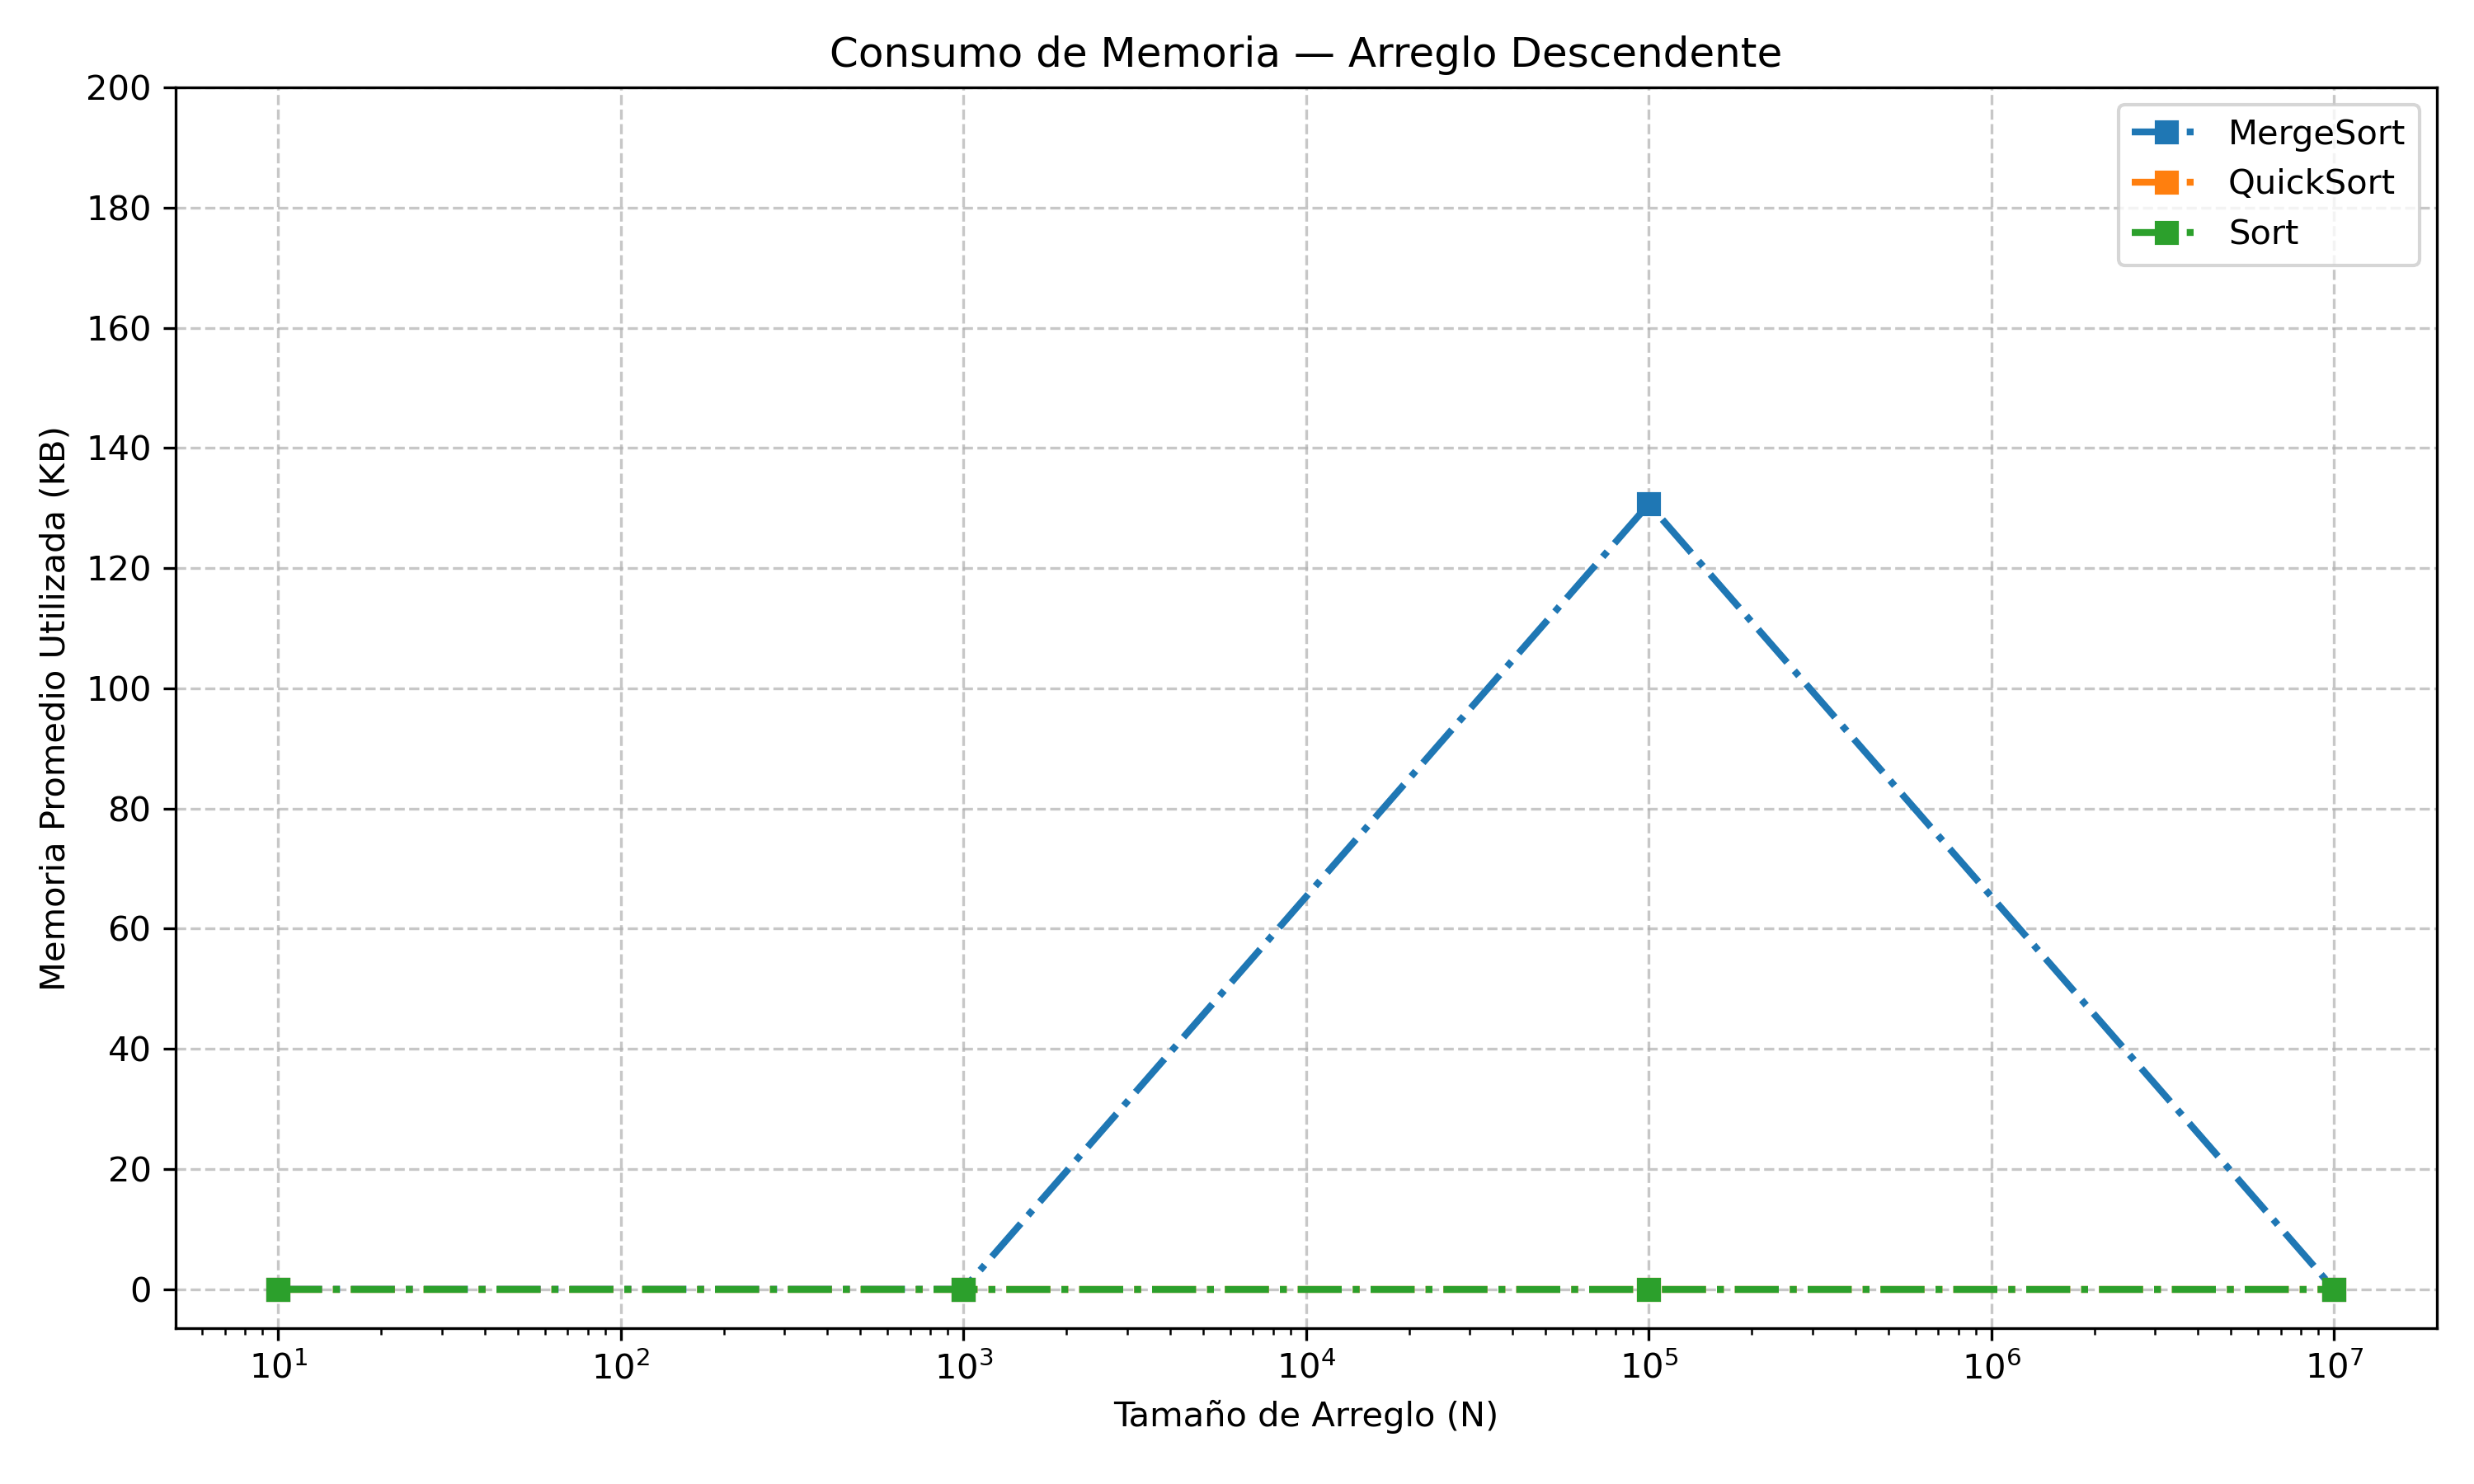
\includegraphics[width=\textwidth]{../code/sorting/data/plots/memoria_descendente.png}
    \end{minipage}%
    \begin{minipage}[t]{0.5\textwidth}
        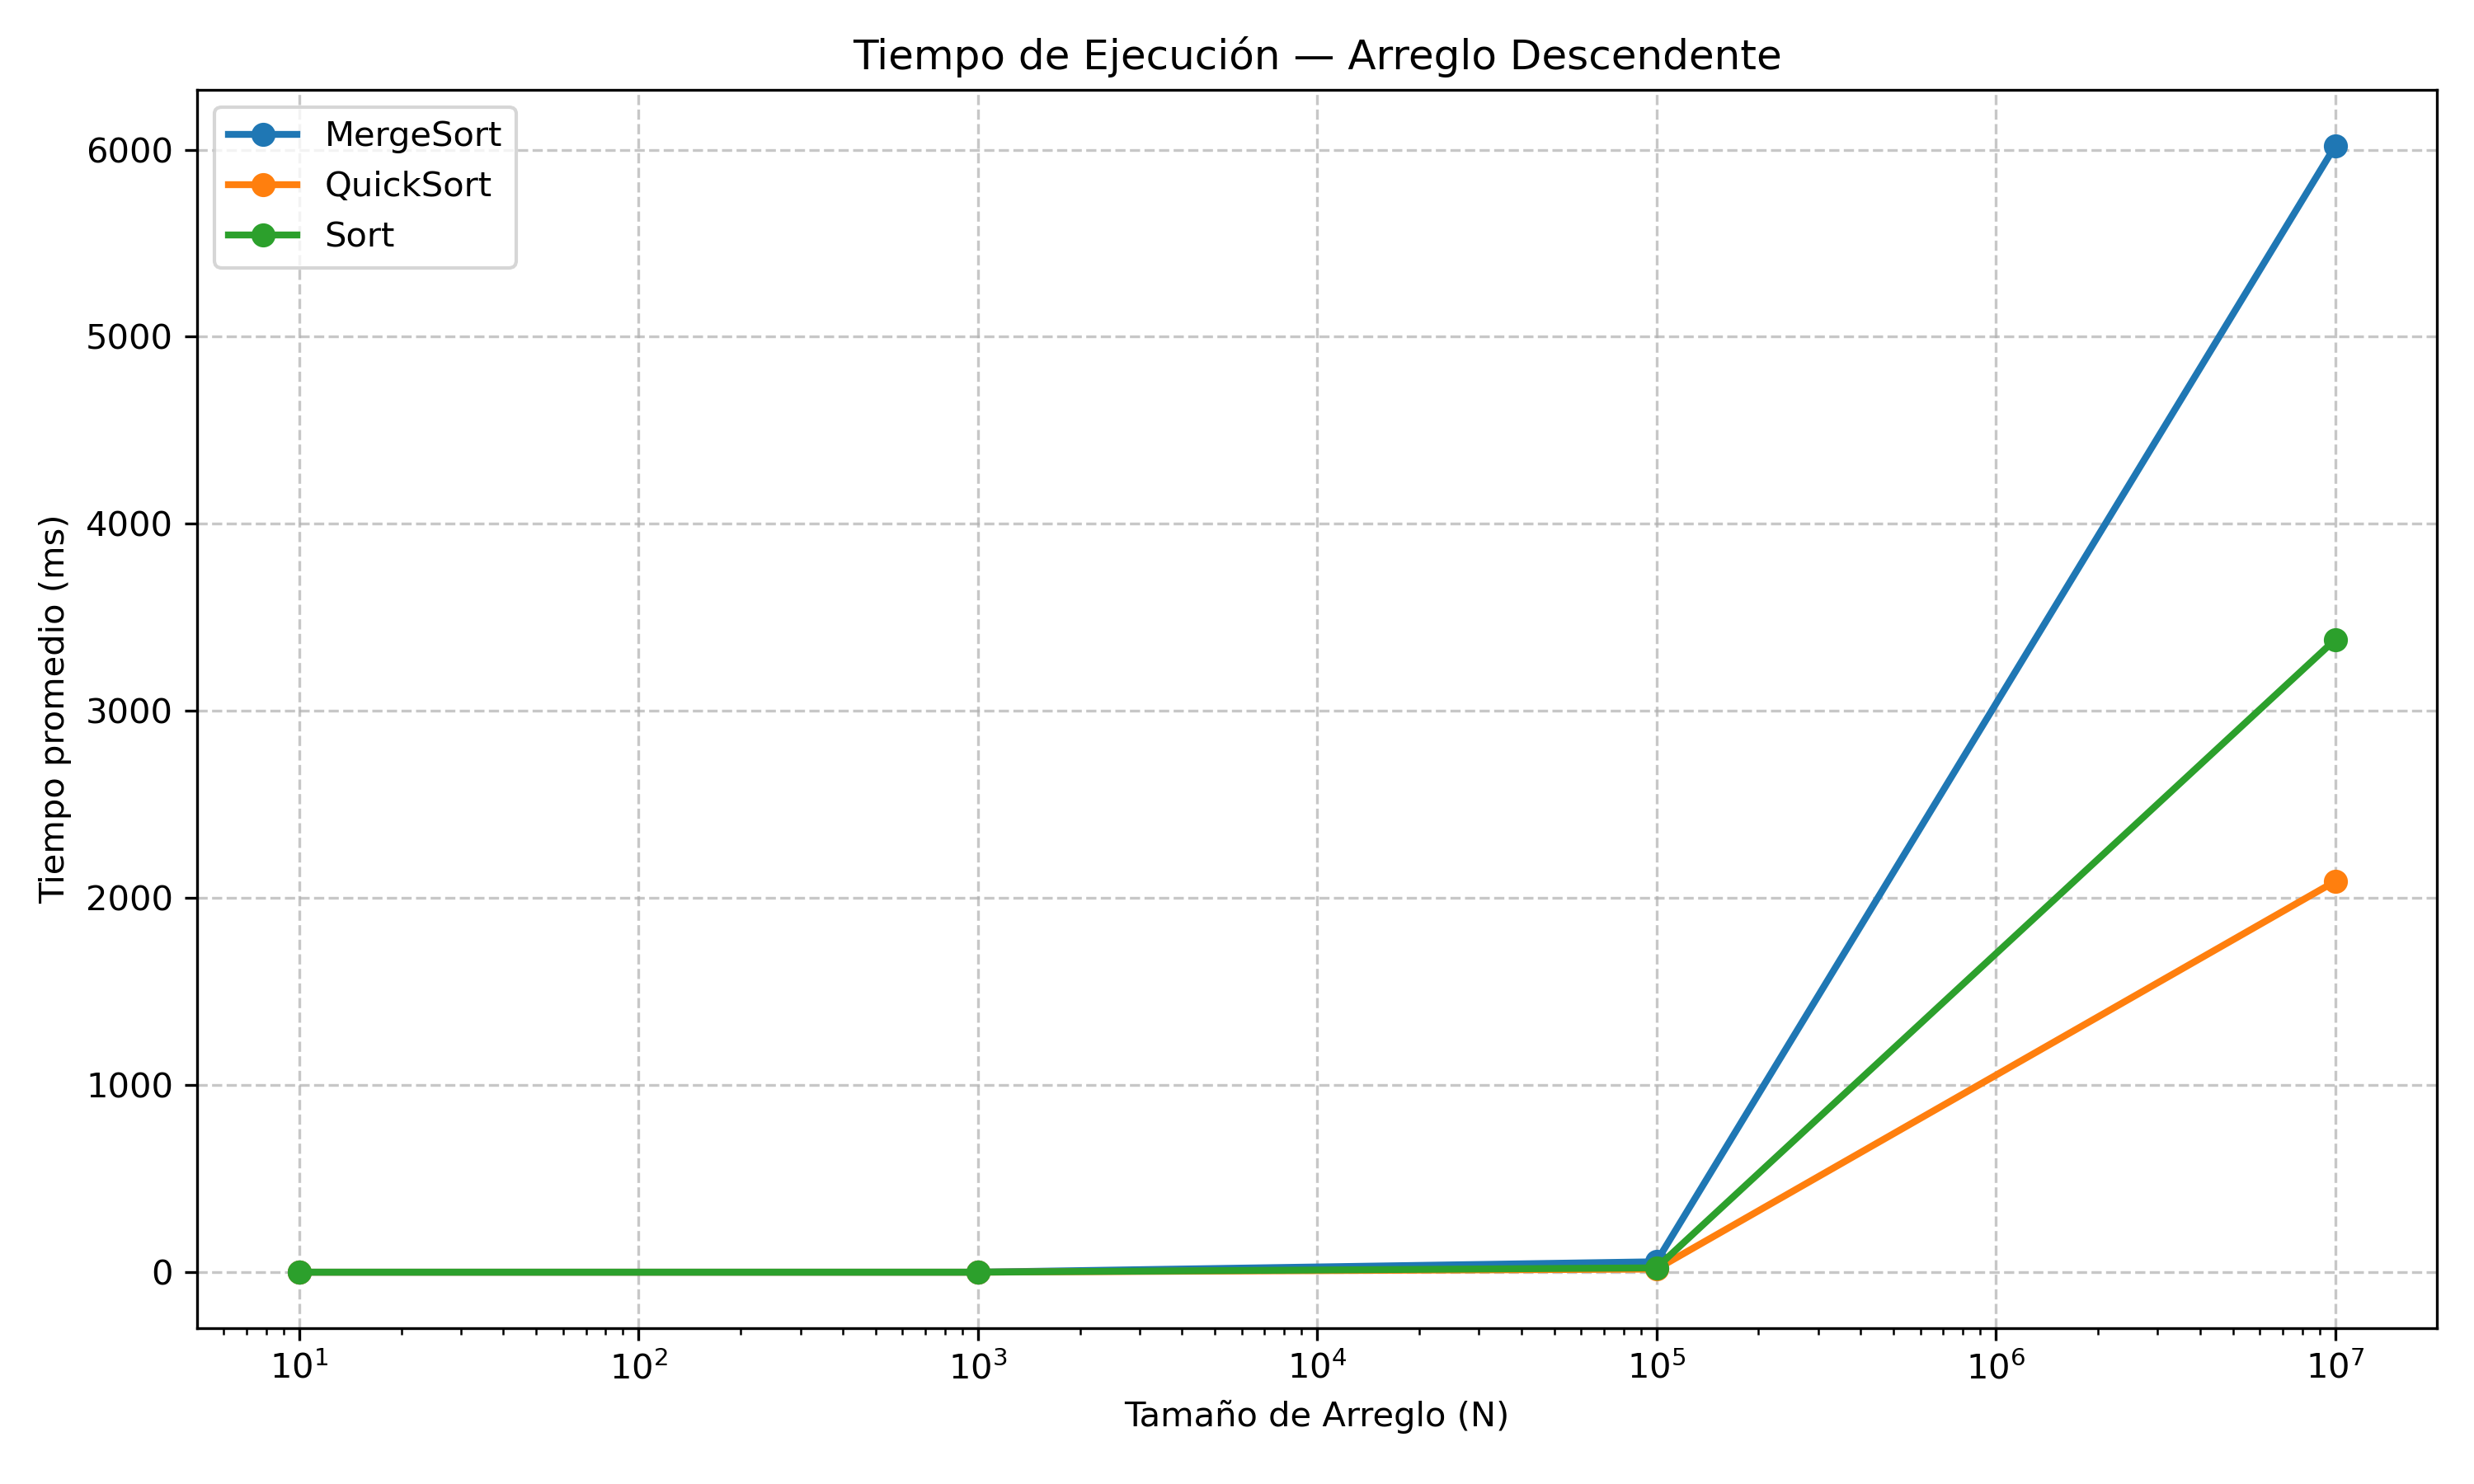
\includegraphics[width=\textwidth]{../code/sorting/data/plots/tiempo_descendente.png}
    \end{minipage}%
    \caption{Comparación del tiempo de ejecución y consumo de memoria de arreglos descendentes por cada algoritmo}
    \label{fig:grafico_descendente}
\end{figure}

En el consumo de memoria tenemos un escenario parecido que, en el caso de los arreglos ascendentes, pues MergeSort posee también un mayor consumo de memoria en arreglos de 100000 y no en los de máximo tamaño, probablemente al motivo explicado antes. Por otra parte, QuickSort y Sort no presentan un consumo notorio en este caso. 

En los tiempos observamos un escenario parecido que, en los arreglos ascendentes, tiempos menores que con los arreglos aleatorios, por lo que una vez más esta reducción pueda deberse a la forma en el que los arreglos estaban desordenados.\\ 

Pasando a los algoritmos de multiplicación de matrices, obtuvimos los siguientes resultados: 

\begin{figure}[H]
    \centering
    \begin{minipage}[t]{0.5\textwidth}
        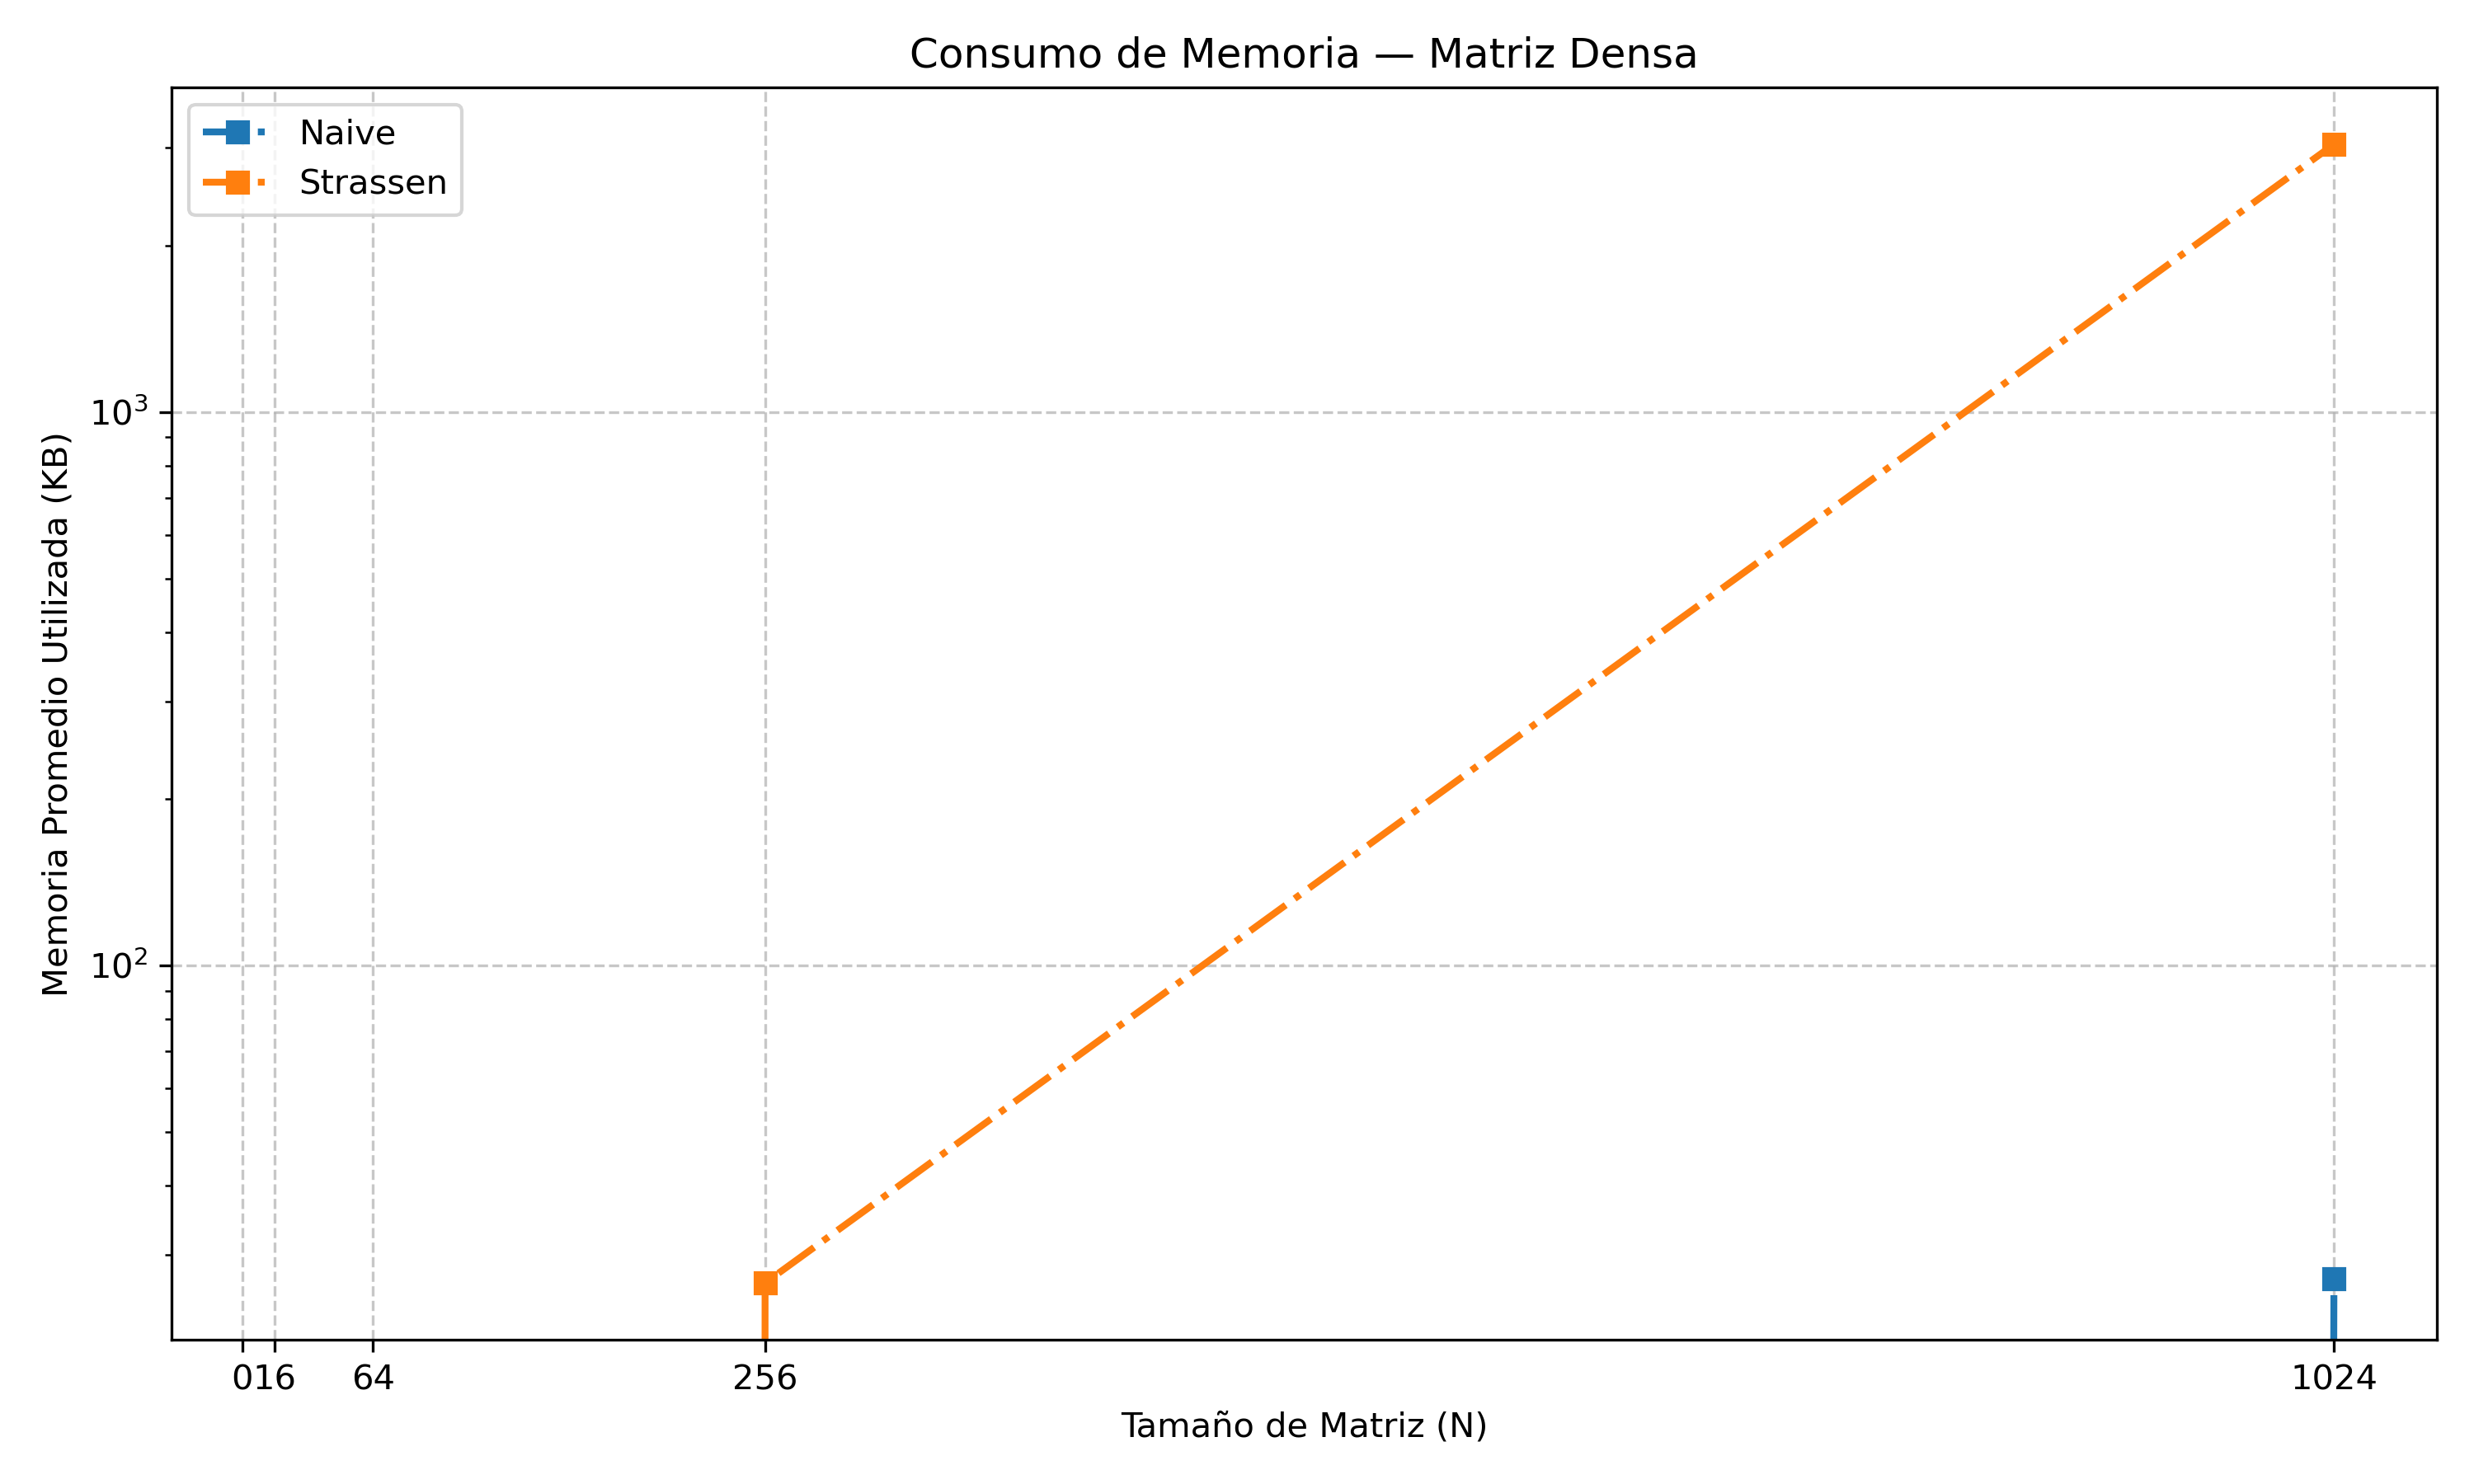
\includegraphics[width=\textwidth]{../code/matrix_multiplication/data/plots/memoria_densa.png}
    \end{minipage}%
    \begin{minipage}[t]{0.5\textwidth}
        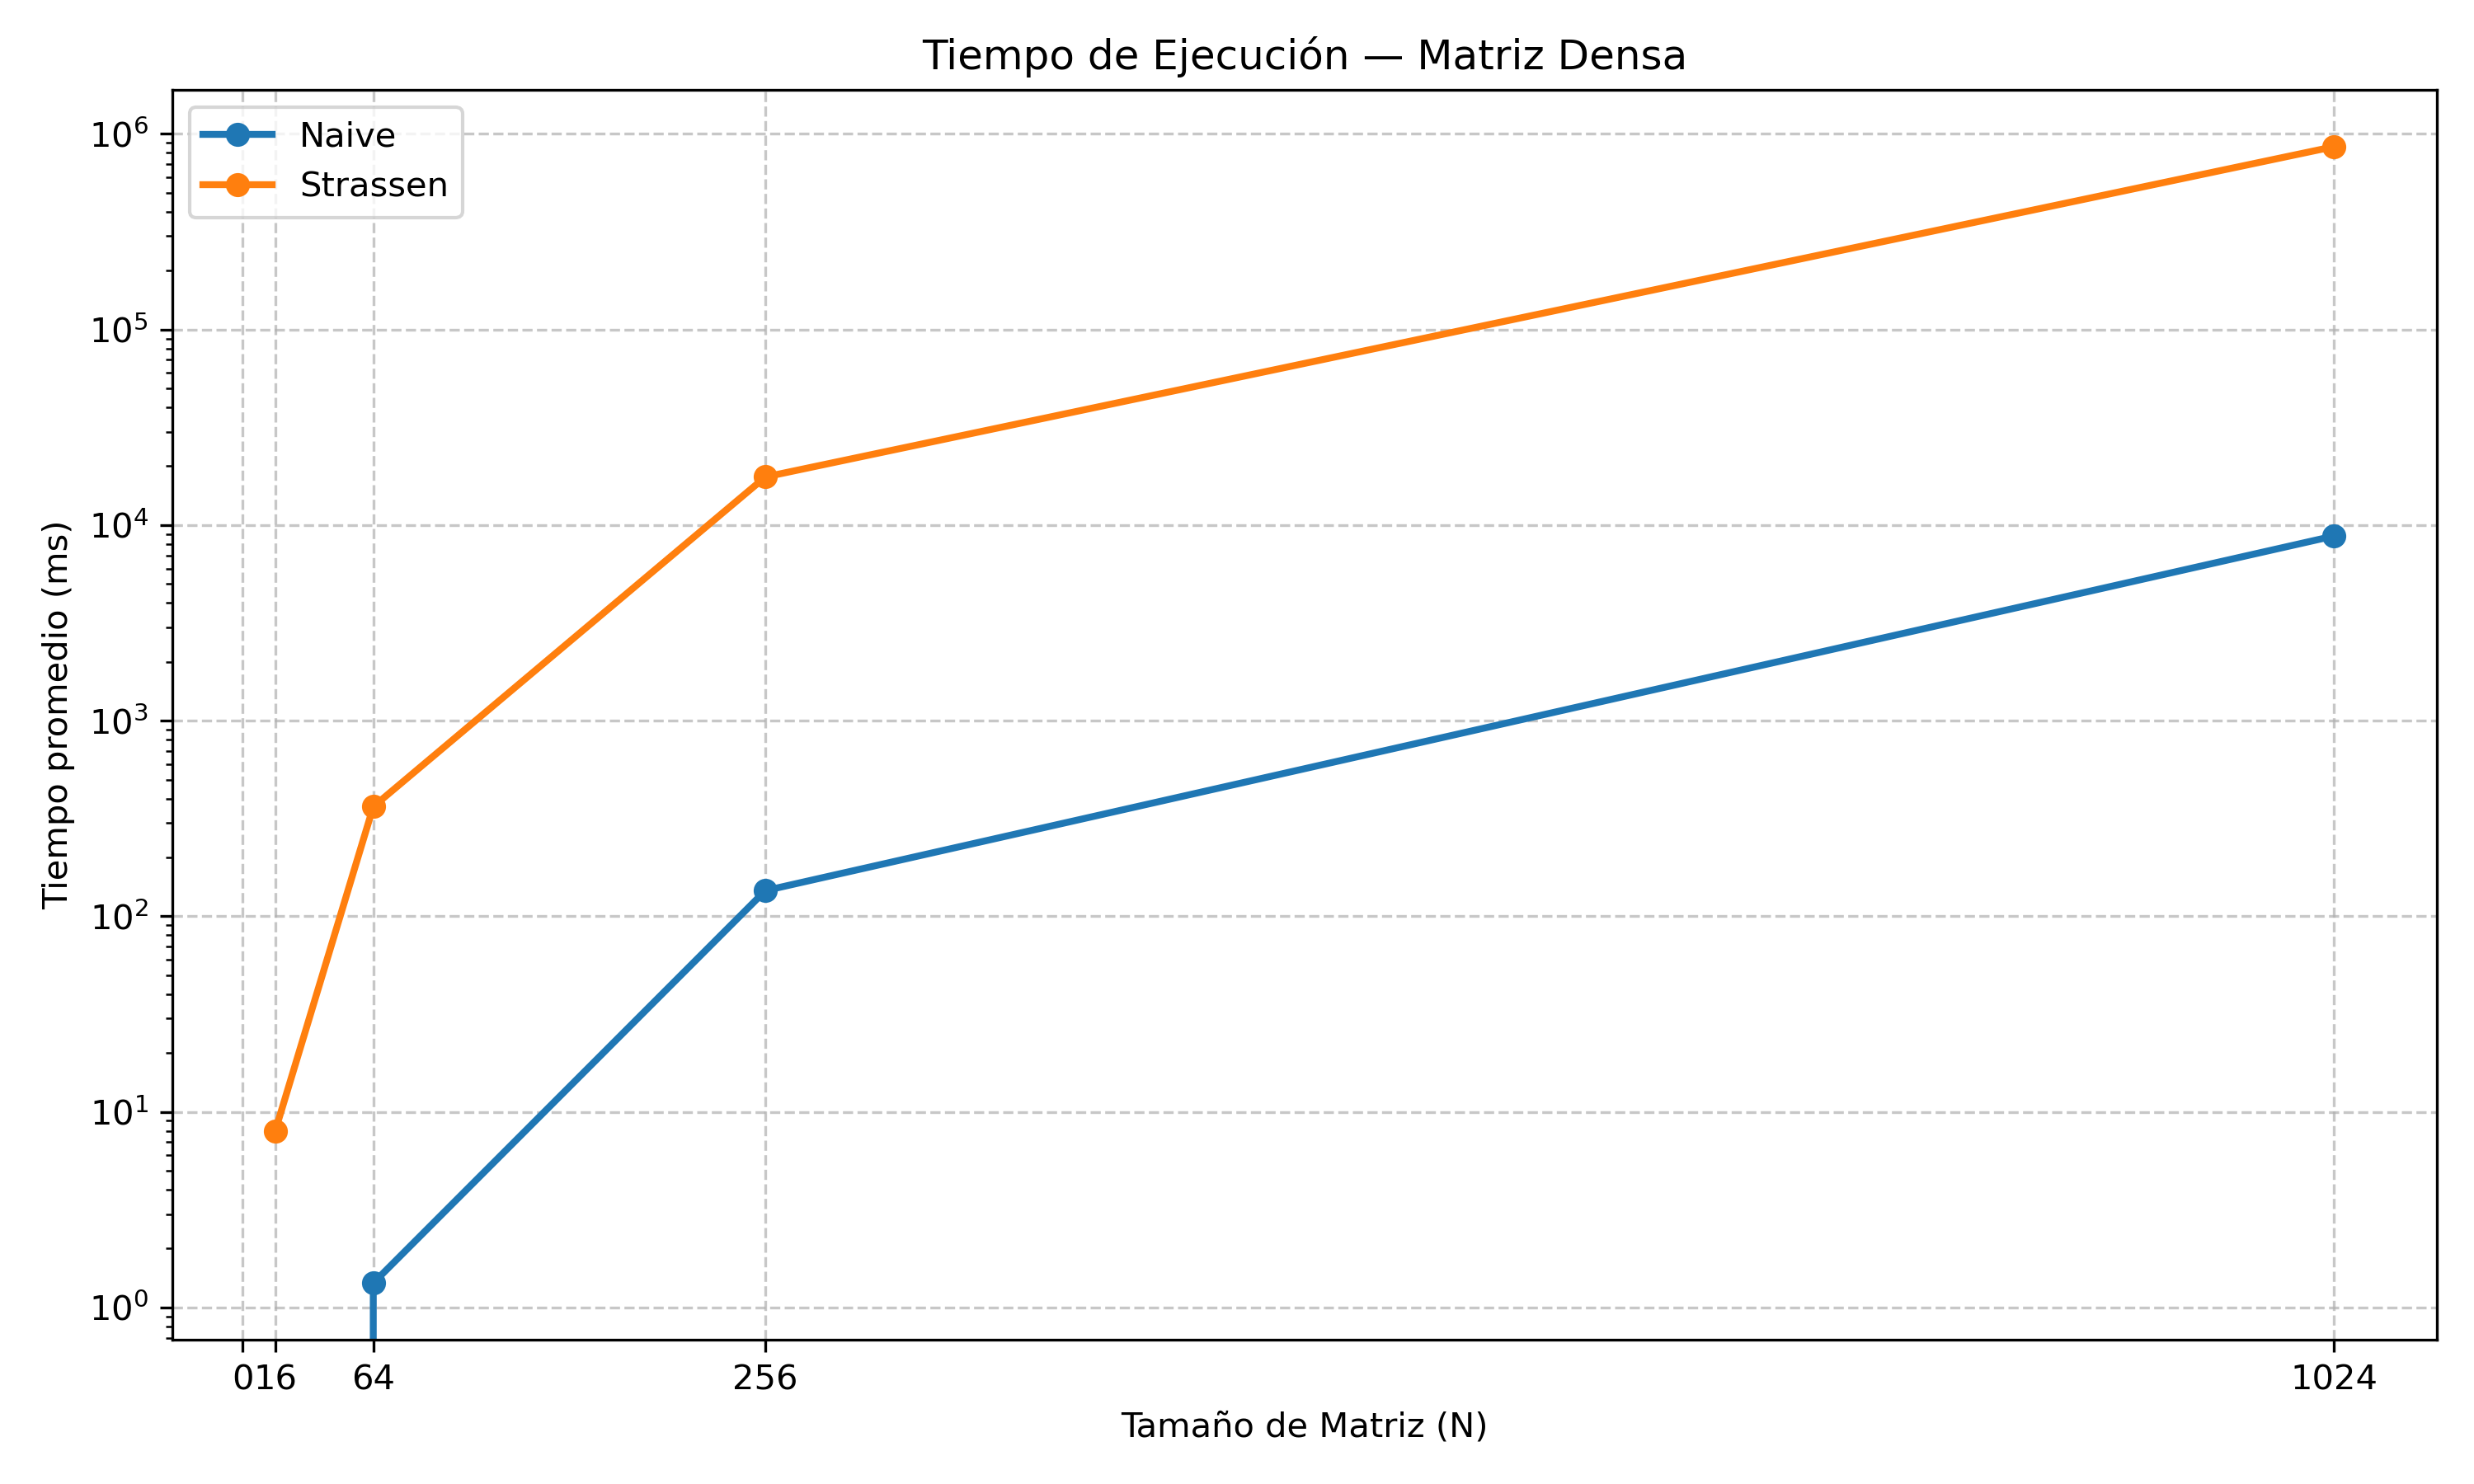
\includegraphics[width=\textwidth]{../code/matrix_multiplication/data/plots/tiempo_densa.png}
    \end{minipage}%
    \caption{Comparación del tiempo de ejecución y consumo de memoria de matrices densas por cada algoritmo}
    \label{fig:grafico_denso}
\end{figure}

Como podemos observar en primera instancia en las matrices densas, el consumo de memoria de straseen es mayor independiente del tamaño de la matriz, esto debido a su enfoque de llamadas recursivas el cual aumenta el consumo de esta misma de forma significativa 

En cambio, naive, al ser un algoritmo de bucles y no recurrir a llamadas recursivas hace que su consumo de memoria sea muy inferior (Al menos para los tamaños tratados en este experimento) 

En cuanto a tiempos de ejecución, nos encontramos con que naive también presenta menores tiempos que strassen, incluso en las matrices de 1024x1024, esto se debe a que Strassen es generalmente mejor cuando se trata de matrices muy grandes, de ahí que naive sea más apto para los tamaños tratados aquí. 

\begin{figure}[H]
    \centering
    \begin{minipage}[t]{0.5\textwidth}
        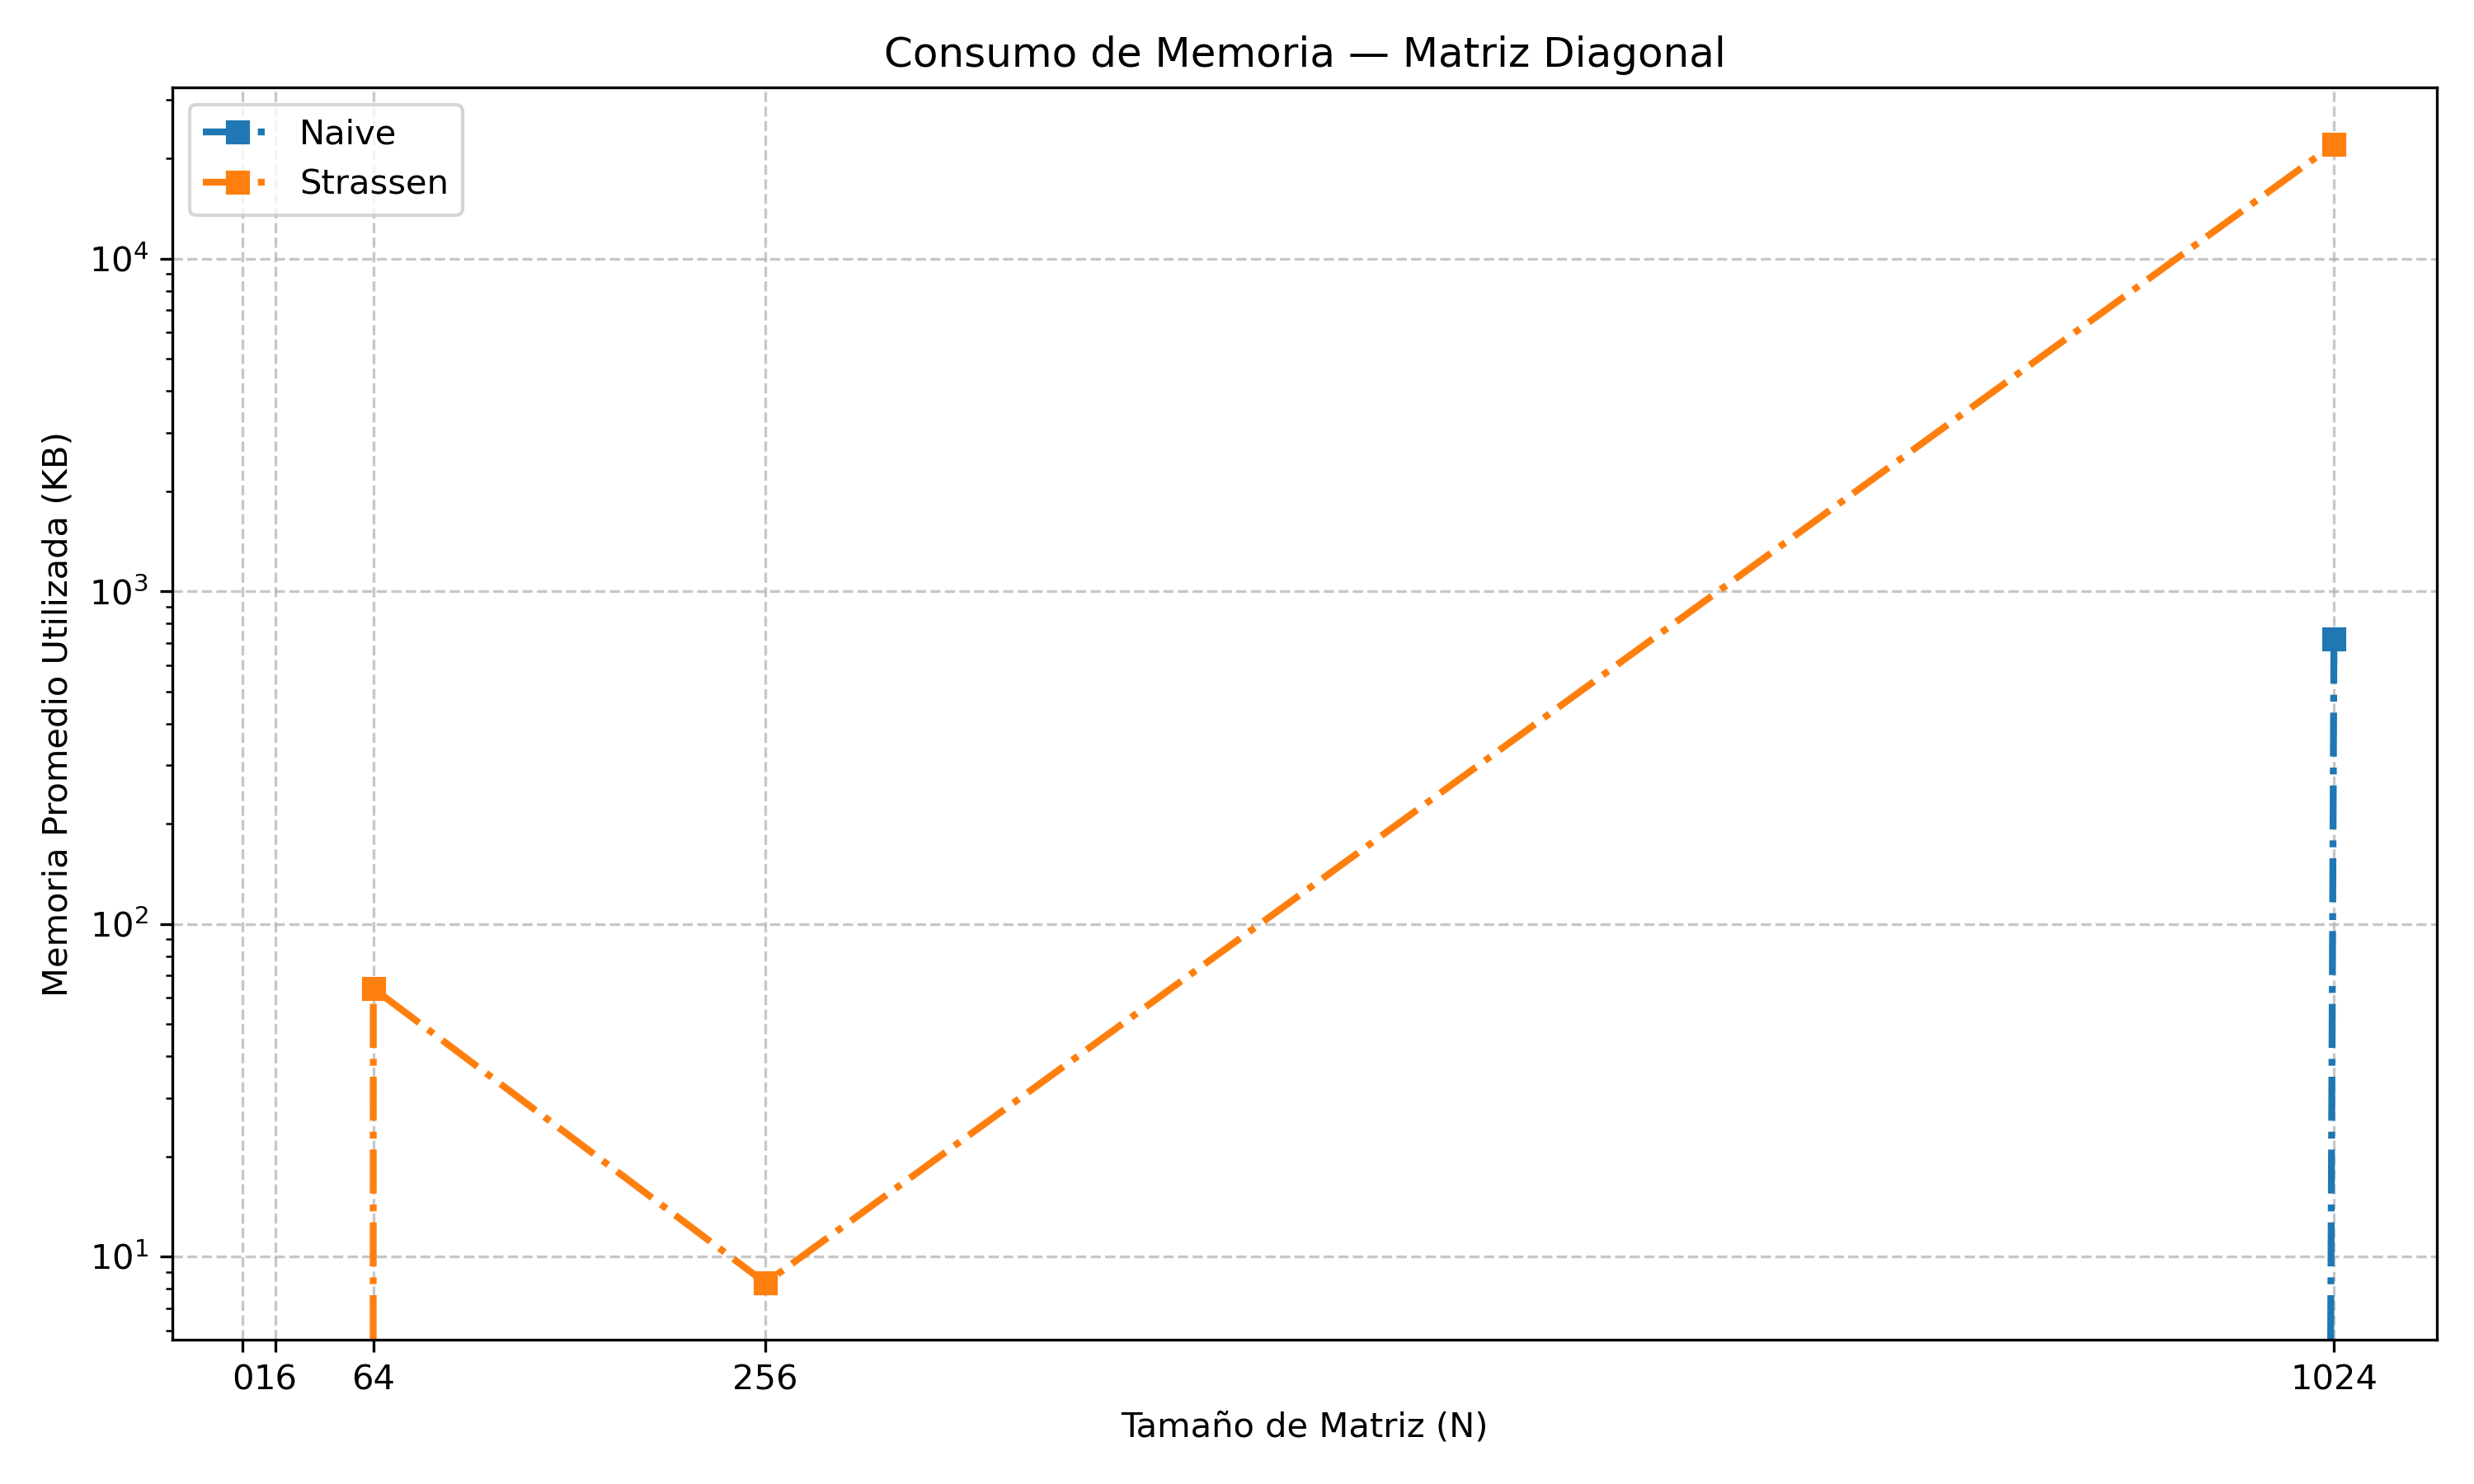
\includegraphics[width=\textwidth]{../code/matrix_multiplication/data/plots/memoria_diagonal.png}
    \end{minipage}%
    \begin{minipage}[t]{0.5\textwidth}
        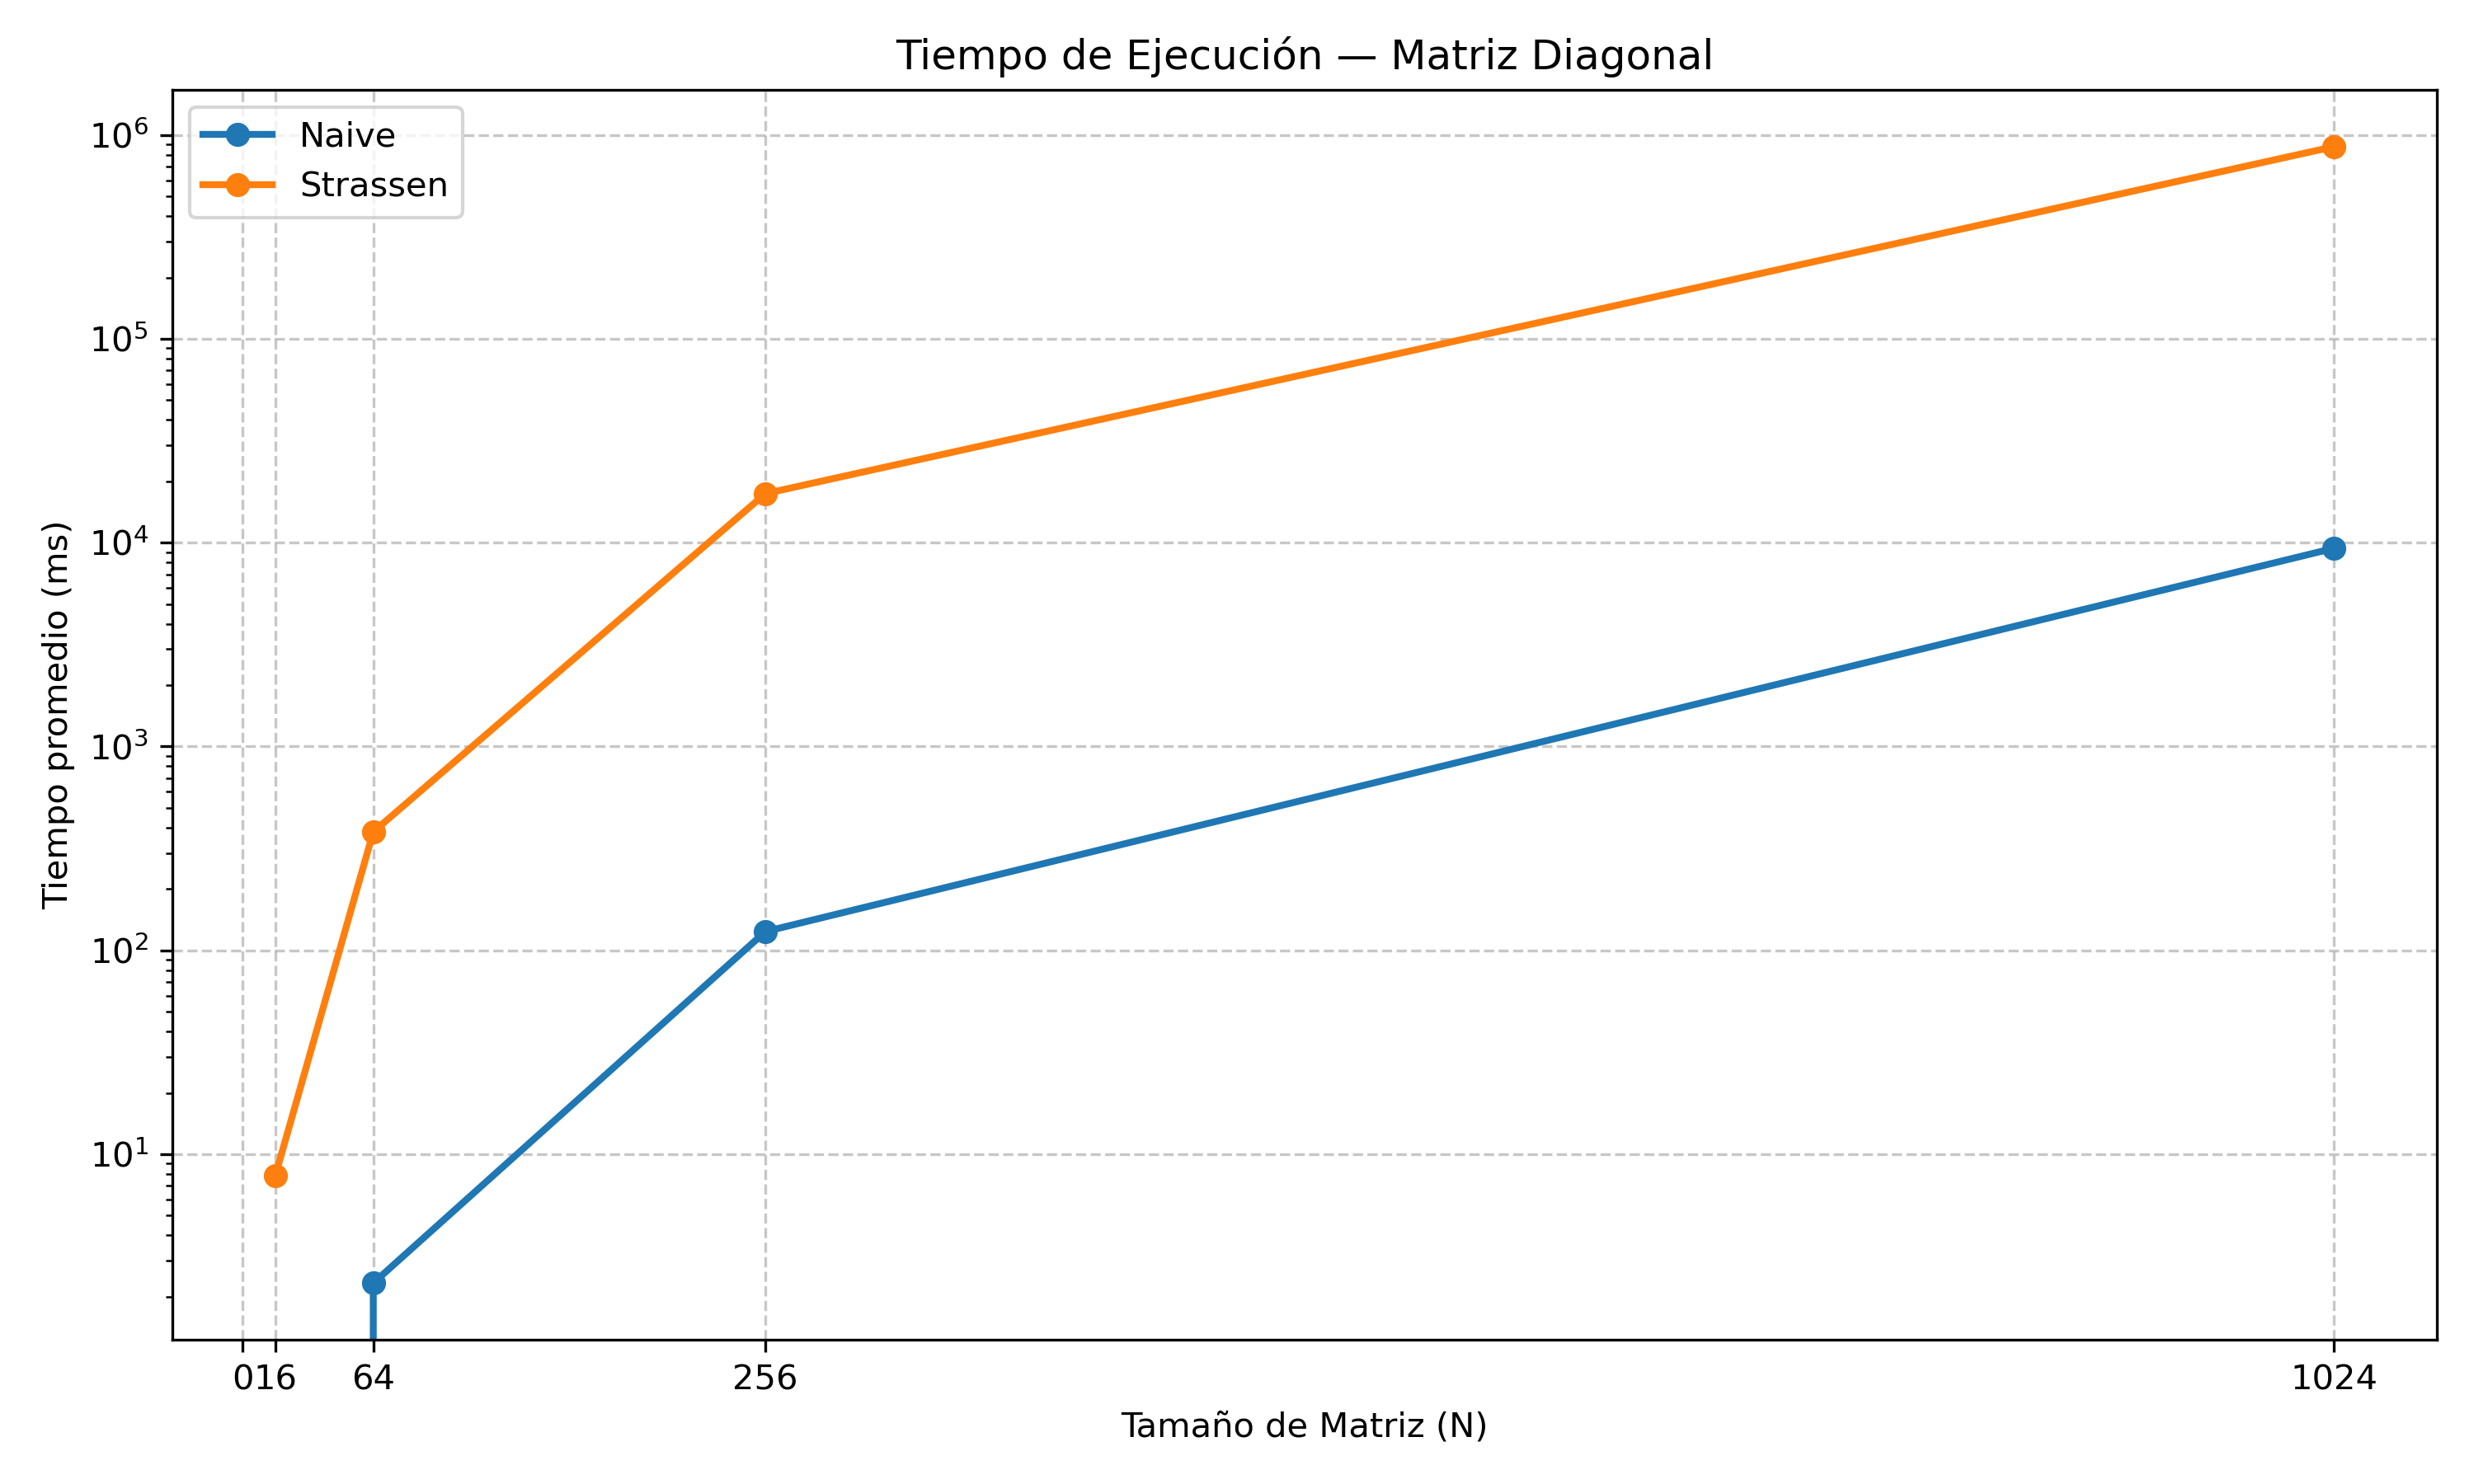
\includegraphics[width=\textwidth]{../code/matrix_multiplication/data/plots/tiempo_diagonal.png}
    \end{minipage}%
    \caption{Comparación del tiempo de ejecución y consumo de memoria de matrices diagonales por cada algoritmo}
    \label{fig:grafico_diagonal}
\end{figure}

Podemos notar que la tendencia se mantiene, strassen en matrices diagonales sigue presentando mayores tiempos de ejecución y memoria que Naive, sin mencionar que acá  
fue donde Strassen presentó el mayor consumo de memoria promedio probablemente por el enfoque de las matrices en cuestión, aunque los tiempos promedio de ambos algoritmos por tamaño se mantienen similares a los de las matrices densas. 

\begin{figure}[H]
    \centering
    \begin{minipage}[t]{0.5\textwidth}
        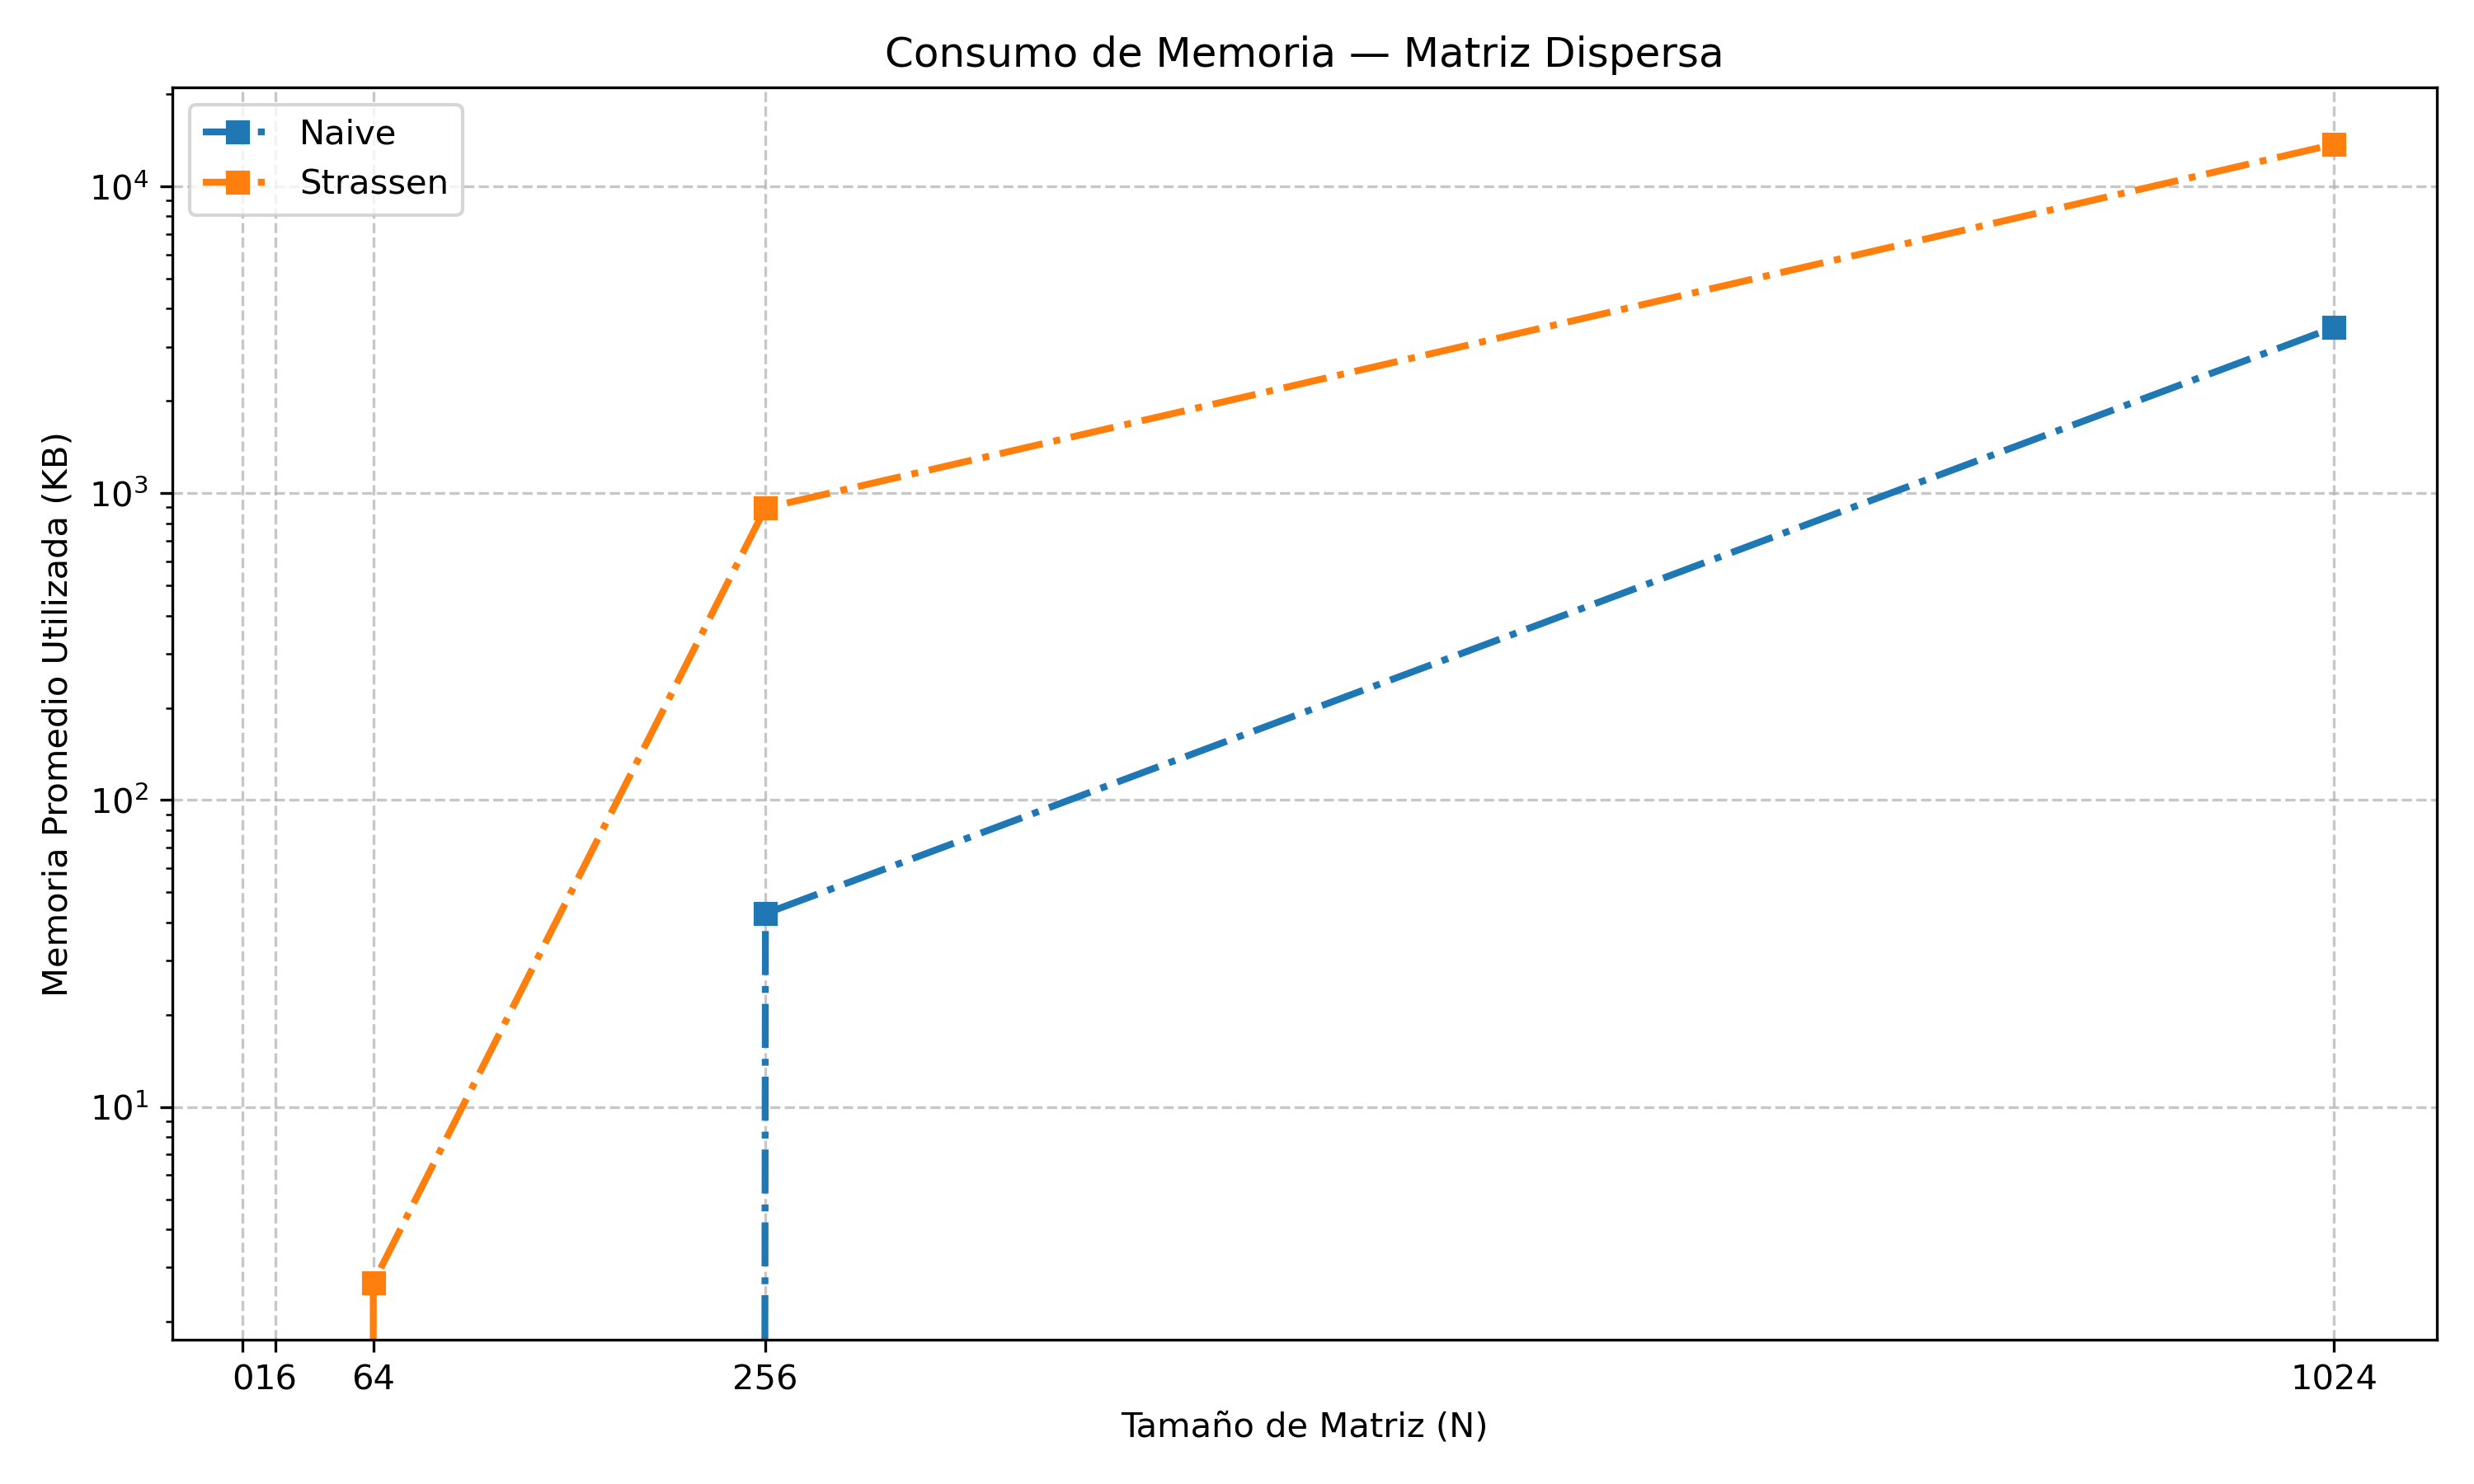
\includegraphics[width=\textwidth]{../code/matrix_multiplication/data/plots/memoria_dispersa.png}
    \end{minipage}%
    \begin{minipage}[t]{0.5\textwidth}
        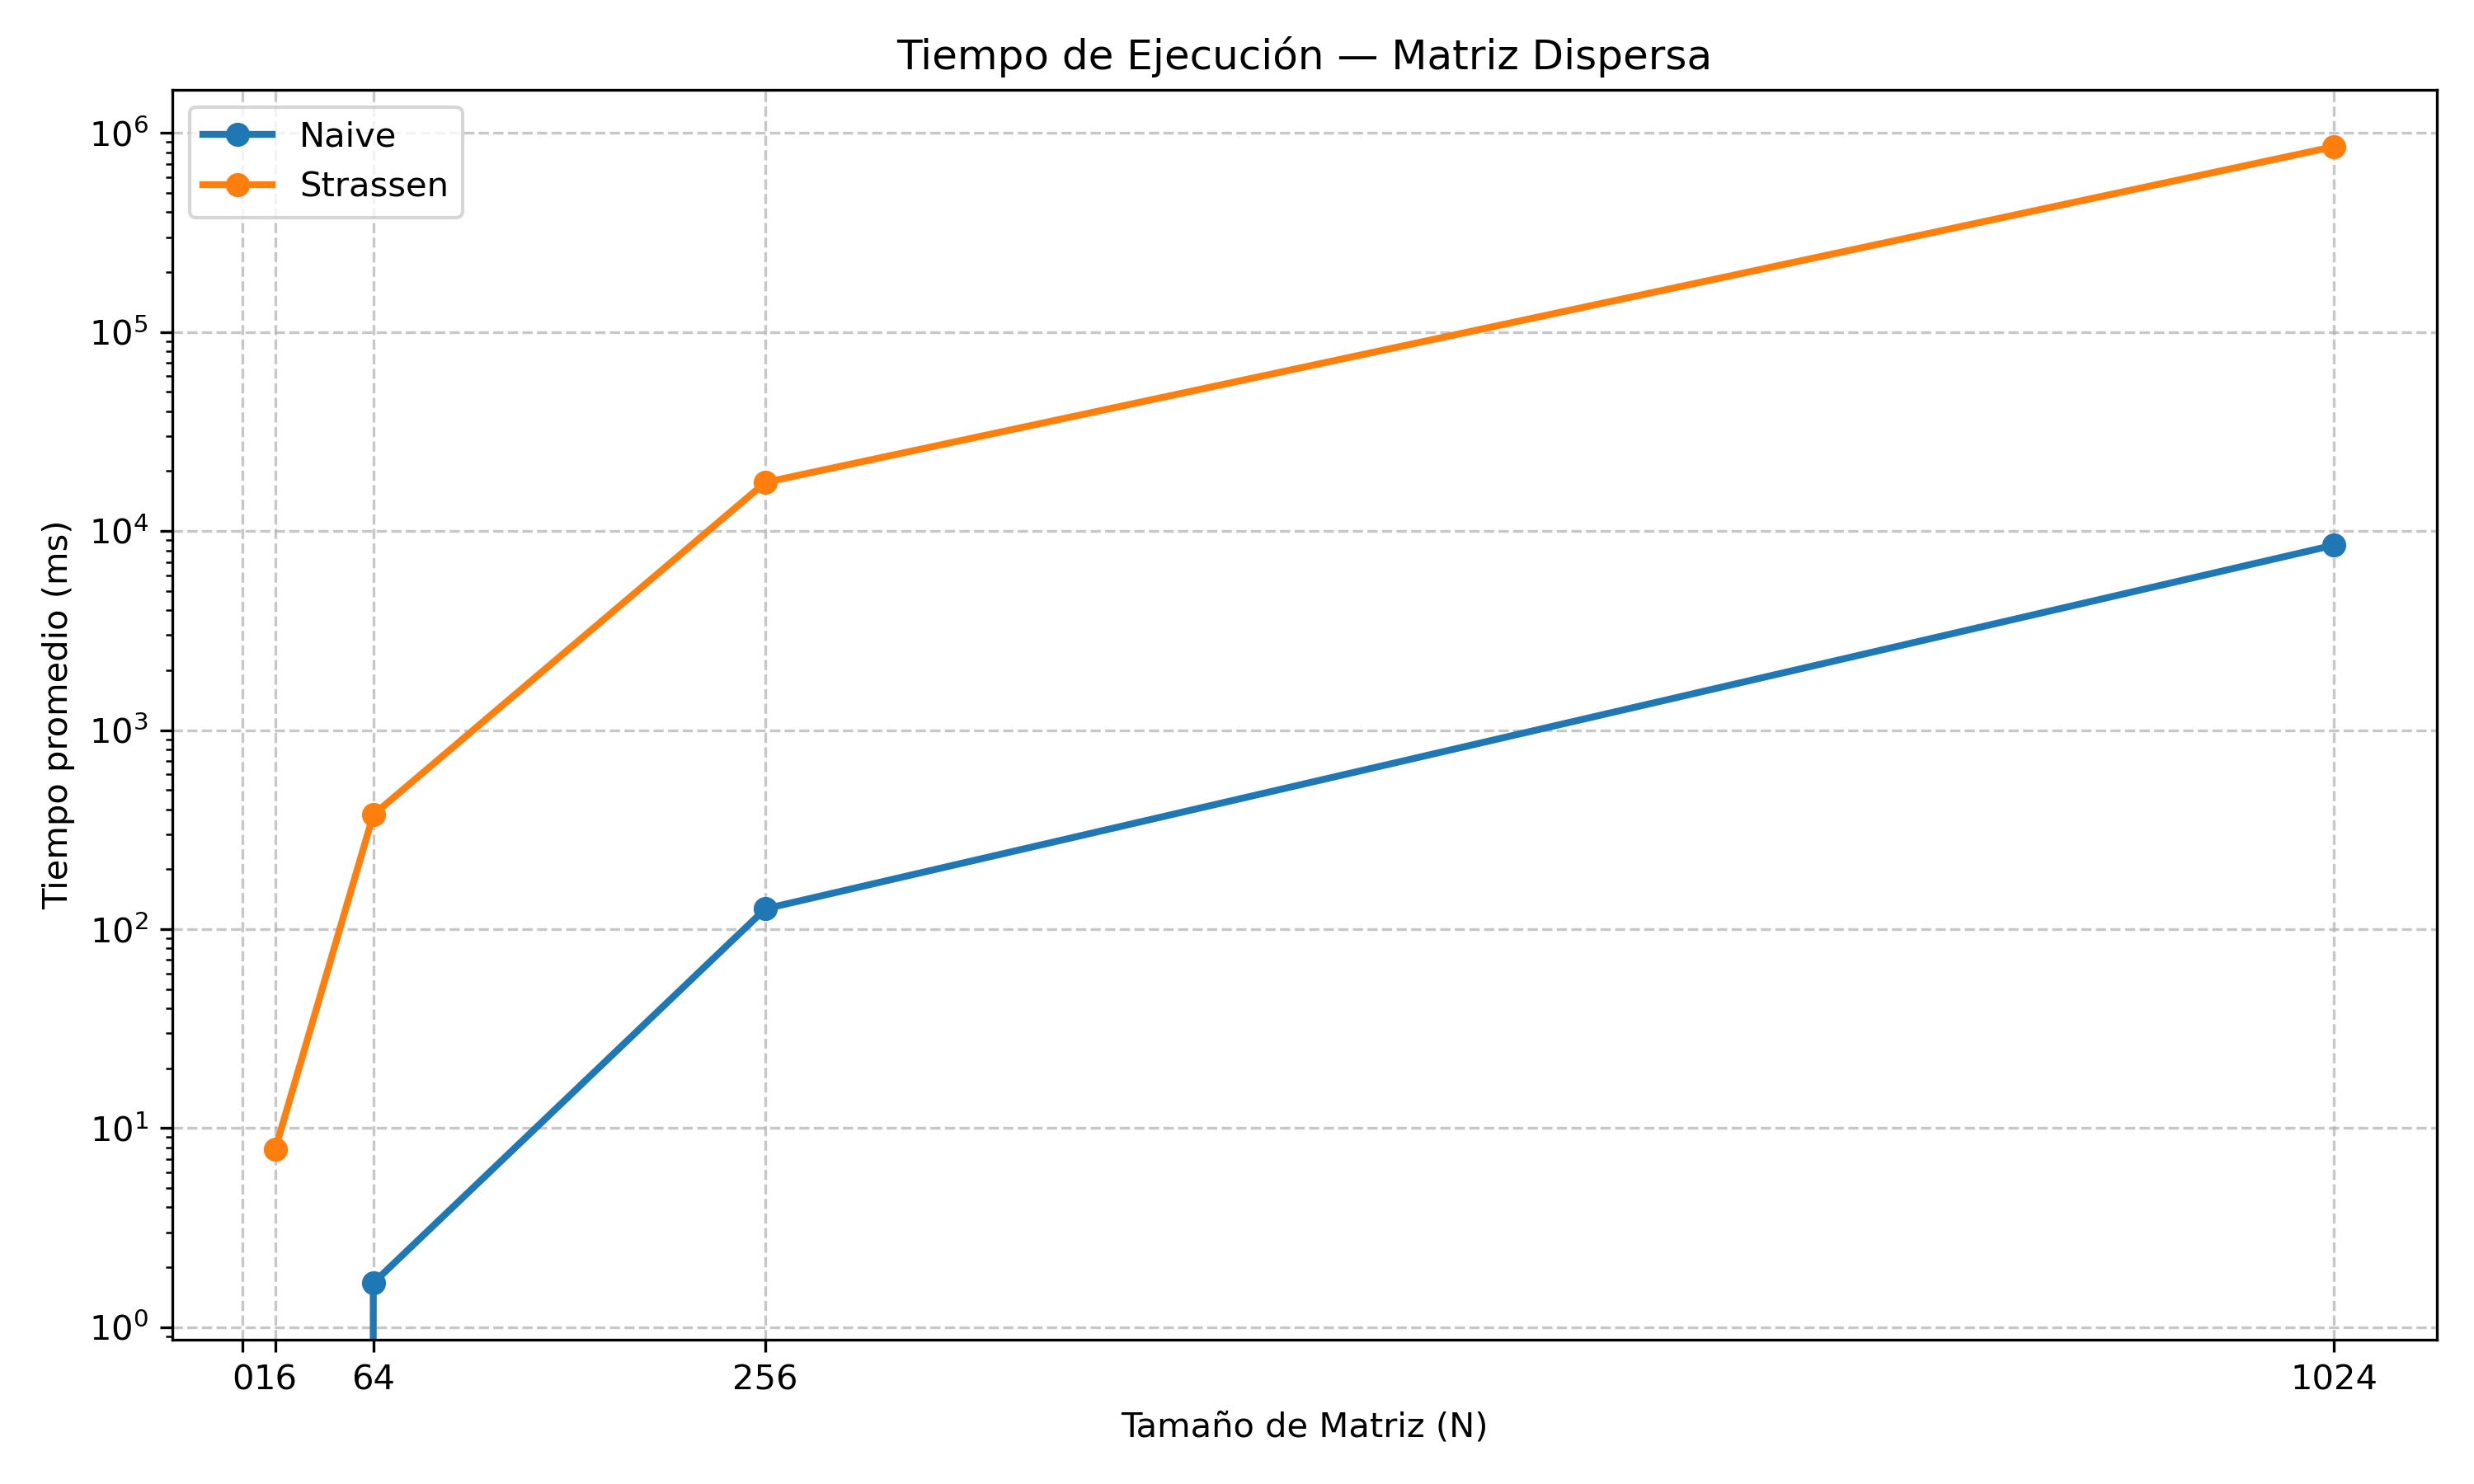
\includegraphics[width=\textwidth]{../code/matrix_multiplication/data/plots/tiempo_dispersa.png}
    \end{minipage}%
    \caption{Comparación del tiempo de ejecución y consumo de memoria de matrices dispersas por cada algoritmo}
    \label{fig:grafico_dispersa}
\end{figure}

Acá se aprecia que el consumo de memoria en strassen se dispara considerablemente a partir de las matrices de 256x256, muy probablemente al orden de estas mismas y que en promedio son capaces de ocupar más espacio de memoria de lo usual a partir de un tamaño más pequeño. 

Naive mantiene la tendencia de bajo consumo de memoria. 

Y en cuanto a los tiempos de ejecución, se mantienen con un promedio similar por tamaño según los gráficos y comparado con los otros tipos de matrices. 
